\documentclass[../main/main.tex]{subfiles}
\begin{document}

% \dominitoc
% \faketableofcontents
% \dominilof
% \fakelistoffigures
% \dominilot
% \fakelistoftables

\chapter{Impact sur la cosmologie~: simulations}\label{ch:sims}
\epigraph{\openquote\textit{The Answer to the Great Question… Of Life, the
    Universe and Everything… Is… Forty-two.}\closequote}{Douglas \textsc{Adams},
    \textit{H2G2}}

Nous avons vu dans le chapitre précédent la manière dont \snana\ permettait de
traiter les biais et corrélations environnementales dans le calcul des
paramètres cosmologiques, et ainsi la raison pour laquelle son utilisation dans
notre thèse était pertinente.

Dans ce chapitre, nous présentons les simulations que nous avons effectuées avec
le logiciel. Dans un premier lieu, nous discutons des différentes corrélations
que nous avons testées \textit{via} l'utilisation de \hostlib\
(Section~\ref{sec:hpres}) et de la confection des nôtres
(Section~\ref{sec:hmake}). Par la suite, nous sondons la qualité de chacun de
ces modèles à décrire les données (Section~\ref{sec:simcomp}) pour finalement
regarder l'impact de ces différentes hypothèses sur la valeur calculée de $w$
(Section~\ref{sec:simres}). Nous concluons Section~\ref{sec:simccl}.

\vfill
\minitoc
\vfill

\newpage

\section{Présentation des \hostlib}\label{sec:hpres}

Dans sa forme la plus générale, une \hostlib\ ne possède pas de valeurs liées à
des paramètres de SNe~Ia (comme l'étirement ou la couleur). En effet, elle sert
originellement à utiliser le redshift photométrique de la galaxie hôte comme
valeur antérieure dans l'ajustement du redshift de la SN et à ajouter du bruit à
la SN simulée (voir Chapitre~\ref{ch:snana}). Avant d'intégrer notre modèle à
\snana, il nous a fallu reproduire les approches d'autres groupes utilisant le
logiciel. Nous avons choisi pour cela les études de~\cite{scolnic2016}, ci-après
SK\defcitealias{scolnic2016}{SK}, et de~\cite{popovic2021a}, ci-après
BP\defcitealias{popovic2021a}{BP}.

\subsection{Étirement et couleur globales~: SK}\label{ssec:sk}

Dans leurs travaux, \citetalias{scolnic2016} n'incluent pas de lien d'étirement
ou de couleur avec les propriétés de la galaxie hôte mais uniquement une marche
de magnitude en fonction de sa masse $M_*$. Celle-ci est incluse dans les
\wgtmap\ des sondages et est de \SI{0.05}{mag}. Le tirage des paramètres $x_1$
et $c$ se font alors depuis des distributions asymétriques Gaussiennes, une par
sondage simulé, décrites par~:
\begin{equation}\label{eq:skasym}
    P(p) = \left\{
        \begin{array}{l}
            e^{-\DS\frac{\abs{p-\mu}^2}{\sigma_-{}^2}
                \quad\text{si}\quad p\leq\mu} \\
            e^{-\DS\frac{\abs{p-\mu}^2}{\sigma_+{}^2}
                \quad\text{si}\quad p>\mu} \\
        \end{array}
        \right.
\end{equation}
avec $p = x_1$ ou $c$. Les valeurs des paramètres sont indiqués
Tableau~\ref{tab:skasym}.

\begin{table}[h]
    \centering
        \caption[Paramètres des distributions d'étirement et de couleur pour les
        simulations SK]{Paramètres des distributions sous-jacentes d'étirement
            et de couleur desquelles sont générées les SNe~Ia dans notre
        reproduction du travail de \citetalias{scolnic2016}.}
        \label{tab:skasym}
    \begin{threeparttable}
        \makebox[\linewidth]{%
        \begin{tabular}{lcccccc}
            \toprule
            \multirow{2}[2]{*}{Sondage} &
            \multicolumn{3}{c}{$x_1$} &
            \multicolumn{3}{c}{$c$}\\
            \cmidrule(lr){2-4} \cmidrule(lr){5-7} &
            $\mu$ & $\sigma_-$ & $\sigma_+$ &
            $\mu$ & $\sigma_-$ & $\sigma_+$ \\
            \midrule
            PS1    &
            0,604  & 1,029 & 0,363   &
            -0,077 & 0,029 & 0,12\\
            SDSS   &
            1,141  & 1,653 & 0,100   &
            -0,038 & 0,048 & 0,079\\
            SNLS   &
            0,964  & 1,232 & 0,282   &
            -0,065 & 0,044 & 0,12\\
            LOWZ   &
            --     & --    & --      &
            -0,055 & 0,023 & 0,015\\
            \bottomrule
    \end{tabular}}
        \begin{tablenotes}[flushleft]
        \item\small \textbf{\hspace{-3,2pt}Notes.} Les valeurs viennent du
            Tableau~1 de \citetalias{scolnic2016}, sauf pour LOWZ dont la
            distribution d'étirement est une double Gaussienne
            d'après~\cite{scolnic2018}.
        \end{tablenotes}
    \end{threeparttable}
\end{table}

Nous avons cependant utilisé les valeurs de paramètres de~\cite{scolnic2018}
pour la distribution d'étirement de LOWZ, qui est alors décrite par une
combinaison de deux Gaussiennes dont une asymétrique, telle que~:
\begin{equation}\label{eq:sklowz}
    P(x_1) = A_1\times
        \left\{
        \begin{array}{l}
            e^{-\DS\frac{\abs{x_1-\mu_1}^2}{\sigma_{-,1}{}^2}
                \quad\text{si}\quad x_1\leq\mu_1} \\
            e^{-\DS\frac{\abs{x_1-\mu_1}^2}{\sigma_{+,1}{}^2}
                \quad\text{si}\quad x_1>\mu_1} \\
        \end{array}
        \right. + A_2\times
        e^{-\DS\frac{\abs{x_1-\mu_2}^2}{\sigma_{2}{}^2}}
\end{equation}
Les valeurs sont indiquées Tableau~\ref{tab:sklowz} avec le rapport d'amplitude
$a=\frac{A_1}{A_2}$. 

\begin{table}[ht]
    \centering
        \caption[Paramètres de la distribution d'étirement pour l'échantillon
        LOWZ des simulations SK]{Paramètres de la distribution sous-jacente
            d'étirement pour l'échantillon LOWZ dans notre reproduction de
        l'étude de~\citetalias{scolnic2016}.}\label{tab:sklowz}
    \begin{threeparttable}
        \makebox[\linewidth]{%
        \begin{tabular}{lcccccc}
            \toprule
            \multirow{2}[2]{*}{Sondage} &
            \multicolumn{6}{c}{$x_1$}\\
            \cmidrule(lr){2-7} &
            $\mu_1$ & $\sigma_{-,1}$ & $\sigma_{+,1}$ &
            $a$ &
            $\mu_2$ & $\sigma_{2}$ \\
            \midrule
            LOWZ &
            0,55 & 1,0 & 0,45  &
            0,55 &
            -1,5 & 0,5 \\
            \bottomrule
    \end{tabular}}
        \begin{tablenotes}[flushleft]
        \item\small \textbf{\hspace{-3,2pt}Notes.} Les caractéristiques sont
            celles reportées dans l'annexe C de~\cite{scolnic2018}, mais les
            valeurs y étant erronées, nous avons utilisé celles de l'équipe
            directement.
        \end{tablenotes}
    \end{threeparttable}
\end{table}

\subsection{Étirement et couleur selon la masse~: BP}\label{ssec:bp}

D'un autre côté, \citetalias{popovic2021a} définissent des distributions mères
Gaussiennes asymétriques pour $x_1$ et $c$ selon la masse de la galaxie hôte.
Ceci est effectué en découpant les données des sondages en intervalles selon
$M_*$~; dans chacun de ces intervalles sont déterminés les paramètres des
Gaussiennes asymétriques, puis à chaque entrée de la \hostlib\ sont sélectionnés
des paramètres d'étirement et de couleur selon la valeur de la masse de la
galaxie hôte. Ainsi, par rapport à SK, ces \hostlib\ présentent deux colonnes
supplémentaires~: une pour $x_1$ et une pour $c$, attribuant à chaque entrée une
valeur de ces paramètres à associer à la SN simulée. 

Ce procédé est réalisé pour LOWZ d'une part, menant à une \hostlib\ que nous
appelons «~BP\_lowz~», et pour la combinaison des sondages DES, SDSS, PS1 et
SNLS d'autre part, menant à une \hostlib\ que nous nommons «~BP\_highz~». Les
valeurs des paramètres correspondants sont disponibles dans l'annexe A2
de~\citetalias{popovic2021a}.

Ce sont ces \hostlib\ qui constituent la base de notre étude~: en réalité, les
\hostlib\ SK sont celles de BP où nous avons retiré le tirage des colonnes $x_1$
et $c$.

\subsection{Étirement selon l'âge~: NN}\label{ssec:nn}

Notre approche des corrélations entre environnement et supernova est une
variation forte par rapport aux précédentes implémentations, puisqu'elle résulte
d'une modélisation prospective plutôt que purement phénoménologique. Pour notre
étude, nous avons besoin de relier l'étirement attribué à la SN avec l'âge de
son environnement, en correspondance avec nos travaux précédents
\citep[][ci-après NN]{nicolas2021}\defcitealias{nicolas2021}{NN}. Nous
augmentons donc les \hostlib\ en faisant correspondre un âge à chaque entrée des
tables. Ainsi, par rapport aux \hostlib\ BP, nous avons donc une colonne
indiquant si la SN est jeune ou vieille, et nommons ces \hostlib\ «~NN~». La
réalisation de cette \hostlib\ est présentée dans la Section~\ref{sec:hmake}.

\subsection{Étirement et marche de magnitude selon l'âge~: NR}\label{ssec:nr}

Comme nous l'avons vu précédemment, l'âge des SNe~Ia a une double implication~:
celle de l'évolution de la distribution sous-jacente de l'étirement avec le
redshift (Chapitre~\ref{ch:stretch}), mais aussi une marche de magnitude de
$\gamma_{\rm env} = \SI{0,13}{mag}$ entre les SNe~Ia jeunes et vieilles
\citep[Chapitre~\ref{ch:stretch},][]{rigault2020}. Nous avons implémenté cette
valeur à la place de la marche de magnitude selon $M_*$ incluse dans les
\wgtmap\ des sondages \textit{via} l'ajout d'une colonne donnant une variation
de magnitude de $\pm\SI{0.065}{mag}$ aux \hostlib\ NN~: ces nouvelles \hostlib\
se nomment «~NR~» pour «~\textsc{Nicolas} \textsc{Rigault}~», et présentent
l'exacte même colonne d'étirement que les NN.

\section{Confection des \hostlib\ NN et NR}\label{sec:hmake}

Afin de simuler des SNe~Ia avec notre modèle, que ce soit pour NN ou NR, nous
avons besoin que les propriétés des galaxies hôtes suivent les distributions de
ce qui a été observé par les différents sondages simulés. Bien que nous
soutenions que le LsSFR est un meilleur traceur de l'environnement d'une SN
\citep{briday2022}, la plupart des sondages caractérisent les galaxies avec leur
masse stellaire. Étant donné que le LsSFR est lié à la masse de la galaxie
hôte\footnote{Pour rappel~: $\mathrm{sSFR} = \frac{\rm SFR}{M_*}$.}, nous ne
pouvons pas uniquement nous baser sur la valeur du redshift $z$ d'une entrée des
\hostlib\ BP pour y assigner un étirement. Nous attendons effectivement que les
galaxies vers $M_*\approx12$ ne contiennent des SNe~Ia vieilles  alors que les
galaxies de $M \gtrsim 7$ n'en contiennent que des jeunes.

Par conséquent, afin de comparer les implications de notre modélisation basée
sur le LsSFR avec ce que les autres sondages ont observé, nous avons dû
modéliser les masses des galaxies hôtes par rapport au LsSFR. Nous avons pour
cela utilisé le même échantillon du Chapitre~\ref{ch:sample} que pour la
modélisation de l'étirement du Chapitre~\ref{ch:stretch}. Cependant, nous
soulignons que cette étude n'a pas pour volonté de décrire l'évolution des
masses des galaxies hôtes (qui sont des propriétés globales) avec le LsSFR d'une
supernova (étant une propriété intrinsèque de celle-ci)~: son utilité est
d'associer de manière cohérente un âge à une SN caractérisée par un certain
redshift et par une masse de galaxie hôte.

\subsection{Modélisation du lien entre masse et redshift}\label{ssec:mmod}

De la même manière que dans le Chapitre~\ref{ch:stretch}, nous utilisons le
LsSFR comme traceur de l'âge d'une SN, mais cette fois sur les estimations de
masse du sondage SNf. Ensuite, nous modélisons les populations jeune et vieille
par une série de paramétrisations différentes et choisissons celle qui a le plus
faible AIC. Cependant, les masses SNf ont été calculées à l'aide de l'Équation~8
de~\cite{taylor2011} (voir~\cite{rigault2020}) alors que d'autres études du
catalogue Pantheon utilisent différentes techniques d'estimation de la masse qui
pourraient donner des valeurs de sortie différentes pour une même galaxie.

L'estimation de \textsc{Taylor} utilise la magnitude AB absolue en bande $i$
d'une galaxie, $M_i$. Elle est déduite de la magnitude apparente $m_i$
connaissant le redshift de la galaxie mais suppose que la bande $i$ observée est
proche de celle du référentiel de repos, ce qui est vrai pour les redshifts de
SNf qui sont inférieurs à $z\approx 0,05$. Les relevés de l'échantillon Pantheon
sont à des redshifts plus élevés et ont utilisé un ajustement des distributions
spectrales d'énergie (en anglais SED pour \textit{spectral energy
distributions}) des galaxies pour éviter les corrections K dans cette procédure.

Nous avons appliqué la même analyse à l'échantillon SNf~: les données ainsi
calculées sont nommées «~SEDSNf~» par la suite et l'échantillon fiduciel
utilisant SEDSNf est nommé «~SED fiduciel~». À cause de l'absence de 4 galaxies
hôtes dans les catalogues de données nécessaires à ce calcul, l'échantillon
SEDSNf est réduit à 110 données, au lien de 114 pour SNf. Nous indiquons
également que nous nous limitons pour cette étude aux galaxies de $M_* >
10^7\si{\Msun}$, étant donné que les valeurs inférieures servent à indiquer
qu'aucune galaxie hôte n'a été définie. L'échantillon fiduciel tombe alors à
548 données, et SED Fiduciel à 544.

Nous avons donc réalisé cette étude de l'évolution des distributions
sous-jacentes de masse avec le LsSFR en utilisant~:
\begin{enumerate}
    \item [\bfseries SNf] Uniquement les données de SNf (masses issues d'un
        calcul par l'Équation de \textsc{Taylor})~;
    \item [\bfseries SEDSNf] Uniquement les données de SNf avec les masses
        issues d'un ajustement par SED~;
    \item [\bfseries Fiduciel] Toutes les données de notre échantillon
        fiduciel~;
    \item [\bfseries SED fiduciel] Toutes les données de notre échantillon
        fiduciel avec les masses SEDSNf.
\end{enumerate}

\begin{figure}[t]
    \centering
    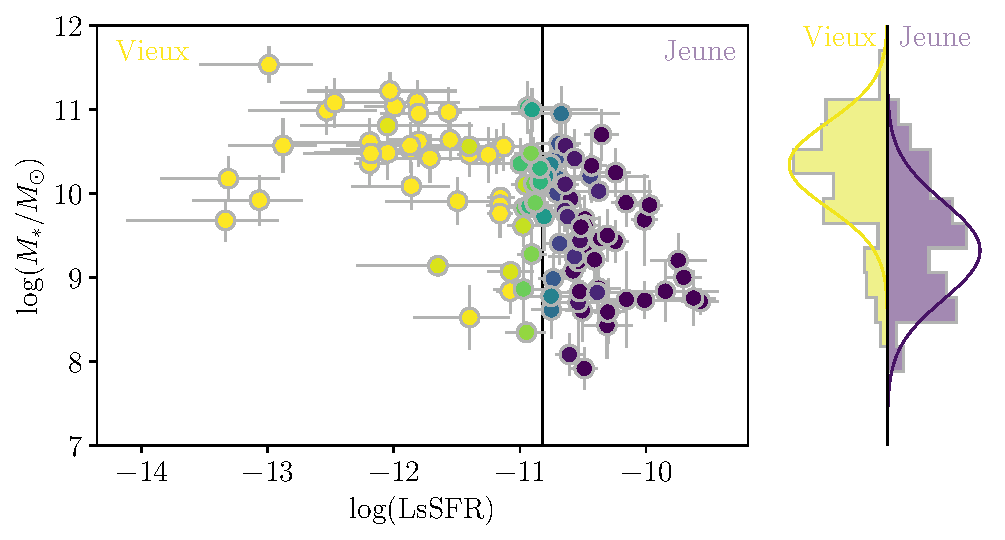
\includegraphics[width=\linewidth]{model_mass_Howell_hist_SED-nonan.pdf}
    \caption[$M_*$ en fonction du LsSFR des SNe~Ia de SNfactory et modèle de
    masse sélectionné ajusté]{\textit{Principal}~: masses des galaxies hôtes
        ($M_*$) ajustées par SED en fonction du LsSFR pour les SNe de SNfactory.
        La couleur correspond à la probabilité $p_y$ que la SN~Ia soit jeune,
        c'est-à-dire qu'elle ait $\log \mathrm{LsSFR} \geq -10,82$
        \citep[voir][et Chapitre~\ref{ch:stretch}]{rigault2020}. \textit{À
        droite}~: histogramme pondéré par $p_y$ des étirements des SNe, ainsi
        que le modèle sélectionné ajusté. Les contributions des populations
    jeune et âgée sont indiquées en violet et jaune, respectivement.}
    \label{fig:massmodel}
\end{figure}

D'après la forme des histogrammes de la Figure~\ref{fig:massmodel}, nous avons
implémenté différentes modélisations. Cette étude étant annexe à la simulation
par \snana, nous ne présentons que les plus pertinentes et omettons les
modélisations n'ayant pas d'intérêt physique ou mathématique, c'est-à-dire les
modélisations constantes avec le redshift (notamment les Gaussienne simple et
Gaussienne asymétrique pure) et les modèles ne convergeant pas. Ainsi, nous
présentons les modèles suivants~:

\begin{itemize}
    \item «~Bi-normal~»\footnote{Même paramétrisation que le modèle
            «~Howell~»~\citep{howell2007} pour le stretch, voir
        Chapitre~\ref{ch:stretch}.}, avec une Gaussienne simple pour chacune des
        populations jeune et âgée~;

    \item «~Normal+asym~» où la population jeune est une simple Gaussienne et la
        population vieille est une Gaussienne asymétrique~;

    \item «~Bi-asym~» où les deux populations jeune et âgée sont asymétriques.
\end{itemize}

\subsection{Comparaison aux données}\label{ssec:mres}

Chacun de ces modèles a été ajusté aux différents échantillons, et nous en
présentons maintenant les résultats. La procédure d'ajustement est celle de la
Section 3 de~\citetalias{nicolas2021}, selon la présence de LsSFR dans chaque
sous-échantillon. Nous définissons de même que précédemment
\begin{equation}\label{eq:likelihood2}
    -2\ln(L) = -2 \sum_i \ln \prob{x_1^i}{\vec{\theta};
    \mathrm{d}x_1^i, y^i}.
\end{equation}
et nous utilisons le critère d'information
d'\textsc{Akaike}~\citep[AIC,][]{burnham2004} pour comparer la capacité de
chaque modèle à décrire correctement les données en pénalisant l'ajout de
paramètres libres tel que~:
\begin{equation}
    \mathrm{AIC} = -2\ln(L) + 2k,
\end{equation}
ce qui permet d'éviter le sur-ajustement. Les résultats sont présentés
Tableau~\ref{tab:modelcomp}.

\begin{table}[h]
    \centerfloat
        \caption[Comparaison de la capacité relative de chaque modèle à décrire
        les données selon l'échantillon d'ajustement]{Comparaison de la
            capacité relative de chaque modèle à décrire les données selon
        l'échantillon d'ajustement.}
        \label{tab:modelcomp}
    \begin{threeparttable}
        \begin{tabular}{lcccccccccc}
            %\hline\hline & & & & & & \\[-0.6em]
            \toprule &
            & \multicolumn{3}{c}{Bi-normal ($k=4$)}
            & \multicolumn{3}{c}{Normal+asym ($k=5$)}
            & \multicolumn{3}{c}{Bi-asym ($k=6$)} \\
            \cmidrule(lr){3-5}\cmidrule(lr){6-8}\cmidrule(lr){9-11}
            Échantillon & N$_{\rm SNe~Ia}$ &
            $-2\ln(L)$ & AIC & $\Delta$AIC &
            $-2\ln(L)$ & AIC & $\Delta$AIC &
            $-2\ln(L)$ & AIC & $\Delta$AIC\\[0.2em]
            %\hline & & & & & & \\[-0.6em]
            \midrule
            SNf & 114 &
            230,0 & 238,0 & -- &
            229,8 & 239,8 & -1,8 &
            229,7 & 241,7 & -3,7 \\
            SEDSNf & 110 &
            223,9 & 231,9 & -- &
            221,4 & 231,4 & 0,6 &
            221,3 & 233,3 & -1,4 \\
            Fiduciel & 544 &
            1534,3 & 1542,3 & -- &
            1534,3 & 1544,3 & -2,0 &
            1531,0 & 1543,0 & -0,7 \\
            SED Fiduciel & 548 &
            1546,6 & 1554,6 & -- &
            1546,5 & 1556,5 & -1,9 &
            1538,7 & 1550,7 & 4,0 \\
            \bottomrule
    \end{tabular}
        \begin{tablenotes}[flushleft]
            \item\small \textbf{\hspace{-3.2pt}Notes.} Pour chaque modèle
                considéré, nous indiquons son nombre
                de paramètres libres $k$, et pour chaque échantillon étudié son
                $-2\ln(L)$ (voir Équation~\ref{eq:likelihood}), son AIC et la
                différence d'AIC ($\Delta$AIC) entre ce modèle et le modèle
                Bi-normal, choisi comme référence car présentant l'AIC le plus
                faible pour 6 comparaisons sur 8.
        \end{tablenotes}
    \end{threeparttable}
\end{table}

Après calcul, le modèle Bi-normal est celui qui se détache le plus, étant celui de
plus petit AIC pour 6 modèles sur 8, et est celui représenté sur la
Figure~\ref{fig:massmodel}. Tous les modèles sont cependant considérés comme
étant de bonnes représentations des données. Nous présentons
Figure~\ref{fig:massmod_comp} une illustration des résultats du tableau
précédent, et Figure~\ref{fig:massmod_all} les représentations graphiques des
modèles implémentés variant en redshift.

\begin{SCfigure}[1][h!]
    \centering
    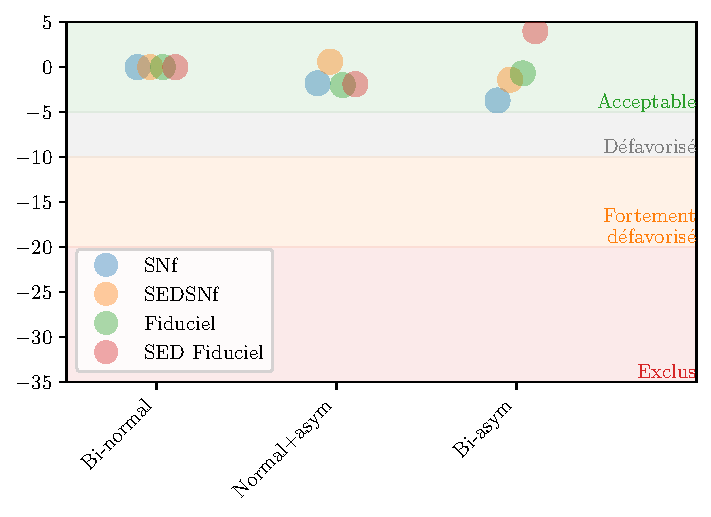
\includegraphics[width=.6\linewidth]{mass_comp_df-nobug}
    \caption[$\Delta$AIC entre le modèle Bi-normal et les autres
    modèles]{$\Delta$AIC entre le modèle Bi-normal et les autres modèles (voir
        Tableau~\ref{tab:modelcomp}). Tous les modèles sont dérivants. Les
        marqueurs bleus, orange, verts et rouges montrent les résultats lorsque
        l'analyse est effectuée sur l'échantillon SNf, SEDSNf, fiduciel,
        fiduciel avec SEDSNf, respectivement (voir légende). Les bandes de
        couleur illustrent la validité des modèles, d'acceptable ($\Delta$AIC >
        -5) à exclu ($\Delta$AIC < -20). En suivant ces valeurs d'AIC, tous les
        modèles sont compatibles entre eux.}
    \label{fig:massmod_comp}
\end{SCfigure}

\begin{figure}[htbp]
    \vspace*{-3cm}
    \centerfloat
    \includegraphics[width=1.1\linewidth]{mass_model_all_evol.pdf}
    \caption[Modèles implémentés et testés dans l'étude de l'évolution de
    l'étirement avec le redshift]{\scriptsize Modèles implémentés et testés dans
        l'étude de l'évolution de la masse avec le redshift. Les modèles
        Bi-normal, Normal+asym et Bi-asym sont tracés dans la colonne de gauche,
        du milieu et de droite, respectivement. Les échantillons sur lesquels
        ils sont ajustés correspondent aux lignes et à la couleur de fond du
        graphique~: SNf (bleu), SEDSNf (orange), fiduciel (vert), fiduciel avec
        SEDSNf (rouge), correspondant aux mêmes couleurs que dans la
        Figure~\ref{fig:massmod_comp}. Les quantités $\Delta(-2\ln(L))$ et
        $\Delta$AIC par rapport au modèle Bi-normal de chaque ligne sont
        indiquées pour chaque modèle figure. Nous avons tracé dix réalisations
        des modèles selon la valeur du redshift moyen considéré, de la valeur la
        plus basse de notre échantillon ($z = 0,02$) à la valeur maximale des
        données totales (sans coupe en redshift) de SNLS ($z = 1,06$). Ces
        modèles sont représentés en couleur allant du jaune (bas redshift, plus
        vieil environnement) au violet (haut redshift, environnement jeune) et
        les distributions des populations jeune et vieille constituant le modèle
        total sont en gris pointillé et fin pointillé, respectivement. Nous y
        retrouvons l'information que tous les modèles sont compatibles en tant
    que bonnes représentations des données par rapport au modèle de base.}
    \label{fig:massmod_all}
\end{figure}

\subsection{Sélection des modèles}\label{ssec:mmodsel}

Avec la multitude de modèles possibles pour établir nos \hostlib, nous avons dû
effectuer une sélection. Étant donné que notre but est d'associer de manière
cohérente un âge de SN définie par un redshift et une masse de galaxie hôte, une
caractéristique primordiale au modèle choisi est d'avoir une évolution de la
fraction de jeunes SNe~Ia physiquement cohérente avec les observations. nous
nous attendons notamment à ce que la fraction de jeunes étoiles soit $\approx$ 1
pour les $M_* \gtrsim 10^7\si{\Msun}$, diminue progressivement jusqu'à $\approx
50\%$ pour $M_* \approx 10^{10}\si{\Msun}$ et continue sa progression vers 0
pour $M_* > 10^{10}\si{\Msun}$~; en effet, la position de la marche de magnitude
basée sur la masse est à $M_* = 10^{10}\si{\Msun}$ et cette limite constitue un
bon indicateur de l'âge d'une SN~Ia d'après~\cite{briday2022}.

Nous avons étudié cette évolution pour les différents modèles implémentés, dont
les résultats sont présentés Figure~\ref{fig:ypc}.

\begin{figure}[ht]
    \centerfloat
    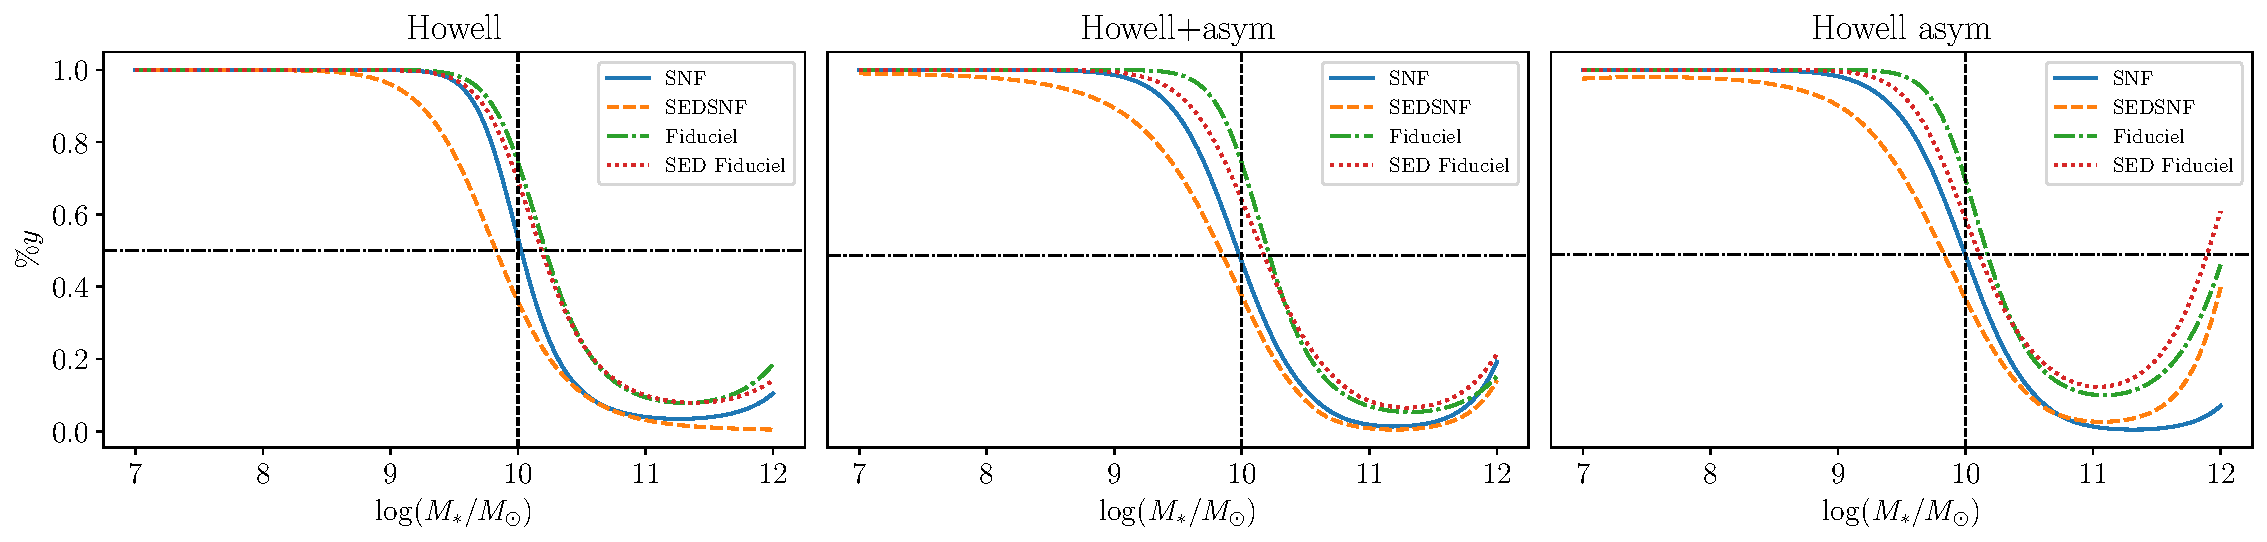
\includegraphics[width=1.2\linewidth]{model_mass_yfrac-best}
    \caption[Comparaison de la prédiction de l'évolution de la fraction de
    jeunes SNe~Ia en fonction de la masse de la galaxie hôte]{Comparaison de la
        prédiction de l'évolution de la fraction de jeunes SNe~Ia ($\%y$) en
        fonction de la masse de la galaxie hôte ($M_*$) pour chaque modèle et
        selon chaque échantillon utilisé pour l'ajustement. Alors que le sens de
        variation devrait être constant, pratiquement tous les modèles finissent
        par remonter après $M_* \approx 10^{11}\si{\Msun}$, sauf le modèle
        Bi-normal ajusté sur SEDSNf. Nous excluons les modèles Normal+asym et
    Bi-asym par ce critère.}
    \label{fig:ypc}
\end{figure}

Nous trouvons alors que tous les modèles finissent par présenter une remontée de
la fraction de jeunes étoiles quand la masse $M_* > 10^{11}\si{\Msun}$, sauf le
modèle Bi-normal ajusté sur l'échantillon SEDSNf. Cela provient de l'incertitude
des courbes Gaussiennes des sous-populations jeunes étant bien plus larges que
celles des sous-populations vieilles, donnant pour les masses élevées un rapport
de probabilité en faveur des jeunes SNe~Ia. Ceci ne correspondant pas à une
réalité physique, nous rejetons tous les modèles Normal+asym et Bi-asym de
notre étude à partir de ces résultats. Parmi les modèles Bi-normal, seul celui
ajusté sur SNf passe en effet par 50\% à $M_*=10^{10}\si{\Msun}$.

Nous conservons ainsi les modèles suivants~:
\begin{enumerate}
    \item Le modèle Bi-normal ajusté sur SEDSNf~;
    \item Le modèle Bi-normal ajusté sur SNf~;
\end{enumerate}
et pour reproduire artificiellement la descente de la fraction de jeunes étoiles
en fonction de la masse attendue, nous avons également~:
\begin{enumerate}[resume]
    \item «~SNfsupp~» («~suppressed~», «~réprimé~»)~: le modèle Bi-normal ajusté
        sur SNf, mais pour lequel les objets de $M_* > 10^{11}\si{\Msun}$ sont
        automatiquement associés à des SNe~Ia âgées. Il ne constitue pas un
        modèle analytique en soit et n'est donc pas tracé Figure~\ref{fig:ypc},
        mais son effet est visible Figure~\ref{fig:fyvMsupp}.
\end{enumerate}

Nous prenons le modèle SNfsupp comme référence. Les implications du choix de
modélisation de masse est discuté Section~\ref{ssec:modsys}. Les valeurs des
paramètres des modèles SEDSNf et SNf sont indiquées
Tableau~\ref{tab:massmodelresults}.

\begin{table}[ht]
    \centerfloat
    \caption[Valeurs des paramètres issus des meilleurs ajustements du modèle
    Bi-normal sur les échantillons SNf et SEDSNf]{Valeurs des paramètres issus
        des meilleurs ajustements du modèle Bi-normal sur les échantillons SNf
    et SEDSNf.}
    \label{tab:massmodelresults}
    \begin{tabular}{lcccc}
        \toprule
        Échantillon              &
                $\mu_{\rm y} $   &
                $\sigma_{\rm y}$ &
                $\mu_{\rm o} $   &
                $\sigma_{\rm o}$ \\
        \midrule
        SNf    & $9.36  \pm 0.06$
               & $0.64  \pm 0.04$
               & $10.58 \pm 0.04$
               & $0.38  \pm 0.04$
               \\
        SEDSNf & $9.32  \pm 0.07$
               & $0.58  \pm 0.05$
               & $10.34 \pm 0.07$
               & $0.51  \pm 0.06$
               \\
        \bottomrule
    \end{tabular}
\end{table}

\subsection{Génération des \hostlib}\label{ssec:inpgen}

Avec les modélisations de la masse et de l'étirement en fonction du redshift,
nous pouvons à présent lire les entrées des \hostlib\ BP, et à partir d'un
redshift générer une liste de masses et d'étirements. Cela nous permettra
ensuite de faire correspondre la masse de la \hostlib\ avec celles de la liste
générée, et d'attribuer une valeur d'étirement qui remplacera celle
de~\citetalias{popovic2021a}.

Cette étape est réalisée avec le module Python
\texttt{SNprop}\footnote{\label{fn:snprop}\href{
    https://github.com/MickaelRigault/snprop}
{https://github.com/MickaelRigault/snprop}}. Ce processus prend la fraction
attendue de jeunes étoiles en utilisant $\delta(z)$ donnée
Équation~\ref{eq:deltaz}. Il assigne une qualité «~jeune~» (LsSFR = 1) ou
«~vieille~» (LsSFR = 0) au tirage qui va suivre en prenant un nombre aléatoire
$r$ entre 0 et 1 et en le comparant à la valeur de la fraction susmentionnée. Si
$r < \delta(z)$, alors la SN simulée sera jeune et inversement. Plus $z$
augmente et plus $\delta(z)$ augmente, et donc plus la probabilité d'être
assignée jeune augmente. Ceci est présenté Figure~\ref{fig:deltaz_rand}.

\begin{figure}[]
    \centering
    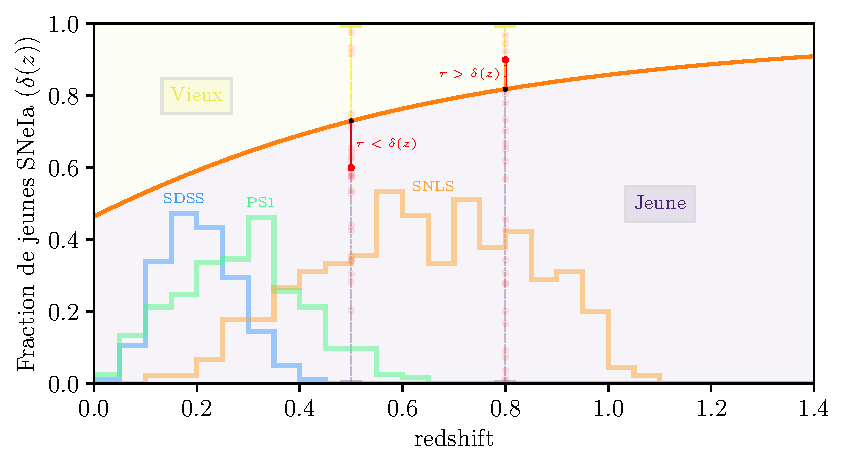
\includegraphics[width=.8\linewidth]{deltaz_hist_yo-random.pdf}
    \caption[Représentation du choix de l'âge d'une SN et de l'assignation de
    masse et d'étirement en fonction du redshift]{Représentation du choix de
        l'âge d'une SN et de l'assignation de masse et d'étirement en fonction
        du redshift du module Python \texttt{SNprop}\footnoteref{fn:snprop}.
        \textit{Orange}~: fraction estimée de jeunes SNe~Ia en fonction du
        redshift. \textit{Histogrammes}~: nombres de SNe~Ia des 3 sondages
        principaux de l'échantillon Pantheon \citep{scolnic2018} (pas à
        l'échelle). \textit{Lignes rouges verticales}~: pour chaque $z$ de la
        \hostlib, un nombre aléatoire $r$ entre 0 et 1 est tiré. S'il est
        supérieur (inférieur) à $\delta(z)$ à ce redshift, alors la SN sera
        assignée vieille (jeune) et les valeurs de masse et d'étirement générées
        seront tirées des distributions sous-jacentes vieilles (jeunes) des
    paramètres correspondants.}
    \label{fig:deltaz_rand}
\end{figure}

Cette étape est réalisée \num{1000} fois pour chaque redshift de la \hostlib,
donnant une table de redshift, âge (0 ou 1), masse et étirement de \num{1000}
entrées, puis une correspondance est effectuée entre toutes les masses tirées et
la masse de la \hostlib\ pour trouver celle qui en est la plus proche. Nous
prenons alors la valeur d'étirement associée et remplaçons celle de la \hostlib.
Au même moment, nous entrons la valeur de l'âge (0 ou 1) dans une nouvelle
colonne~; ceci conclut la confection des \hostlib\ NN.

Les \hostlib\ NR possèdent un autre colonne supplémentaire, où à chaque valeur
d'âge est associée une valeur de variation de magnitude, de +\SI{0,065}{mag}
pour les jeunes (moins lumineuses) et de -\SI{0,065}{mag} pour les vieilles
(plus lumineuses), qui remplacent les valeurs de marche de magnitude basées sur
la masse implémentées dans les autres approches et qui sont associées au
\wgtmap.

\subsection{Implémentation}\label{ssec:snaimpl} 

Nous pouvons implémenter différentes manières d'effectuer ces simulations, que
nous appelons «~types~». Une approche serait de simuler 100 fois des
échantillons de la taille de l'échantillon de Pantheon ($\approx \num{1000}$) et
de combiner les résultats, permettant ainsi d'avoir des incertitudes
statistiques réalistes. Bien que nous ayons entamé la réalisation d'une telle
approche, le plus simple et moins chronophage a été de simuler un échantillon
d'une taille conséquente ($\approx \num{13 000}$) avec un BiasCor cinquante fois
plus grand, donnant une idée de l'incertitude systématique due aux différents
modèles de corrélations (SK, BP, NN, NR).

Pour quantifier cela, nous conservons les données simulées et les échantillons
BiasCor associés de chaque modélisation, afin d'utiliser les données d'un modèle
et de les corriger avec le BiasCor d'un autre~: l'idée derrière cette pratique
est d'évaluer le potentiel biais dû au fait de méconnaître la physique réelle
qui régit les propriétés intrinsèques des SNe~Ia. Pour les distinguer, nous les
nommons de la manière suivante~:
\begin{center}
    \begin{tikzpicture}[]
        \node[anchor=center] (name) at (0,0)
            {\textcolor{cornflowerblue}{SK}\_\textcolor{limegreen}{NR}};
        \node[inner sep=0] (datab) at ([shift={(0,3pt)}]name.south west) {};
        \node[inner sep=0] (biasb) at ([shift={(0,3pt)}]name.south east) {};
        \node[below left =of datab, color=cornflowerblue] (data)
            {Données};
        \node[below right=of biasb, color=limegreen] (bias)
            {BiasCor};
        \draw[-stealth] (data) -- (datab);
        \draw[-stealth] (bias) -- (biasb);
    \end{tikzpicture}
\end{center}
Ainsi, «~SK\_NR~» décrit un échantillon dont les données ont été générées en
supposant les modèles de corrélations de~\citetalias{scolnic2016} et corrigées
avec des données générées en supposant les modèles de corrélations dus à l'âge
(NR). Lorsque les données et BiasCor sont les mêmes, nous ne mentionnons pas
quel est le BiasCor. 

Pour comparer de manière cohérente les données simulées aux données réelles, il
faut que le ratio des données de chaque sondage de l'échantillon simulé
corresponde au ratio des données de chaque sondage de l'échantillon réel. Ceci
s'effectue \textit{via} un paramètre appelé \texttt{NGEN}, décrivant le nombre
d'années de sondage simulé. Il permet de contrôler plus ou moins précisément le
nombre de SNe~Ia simulées, puisque chaque sondage a sa propre efficacité
spectroscopique qui, à chaque simulation, opère une sélection des données
conservées (voir Chapitre~\ref{ch:snana}). Notamment, puisque l'efficacité
spectroscopique de l'échantillon LOWZ est particulièrement faible, il nécessite
un grand \texttt{NGEN} dans nos fichiers de configurations. De plus, la
correction par \bbc\ réduit l'échantillon en ne conservant que les données qui
sont dans un intervalle de BiasCor avec suffisamment de points pour avoir une
valeur de correction. Nous indiquons dans le Tableau~\ref{tab:ratio} le
nombre de données pour les données réelles et pour nos simulations, exprimées en
pourcentages de l'échantillon Pantheon.

\begin{table}[ht]
    \centerfloat
        \caption[Nombre de données de nos différentes simulations]{Nombre de
            données après l'ajustement par \bbc\ et après
            l'échantillonnage nécessaire à la reproduction des ratio
        observés dans l'échantillon Pantheon \citep{scolnic2018}.}
        \label{tab:ratio}
    \begin{threeparttable}
        \makebox[\linewidth]{%
        \begin{tabular}{ccccccc}
            \toprule & &
            \multicolumn{5}{c}{Après \bbc} \\
            \cmidrule(lr){3-7}
            Données & BiasCor &
            Total (/1022) & LOWZ & SDSS & PS1 & SNLS \\
            \midrule
            \multicolumn{2}{c}{Pantheon} &
            1022 (1.00) & 172 & 335 & 279 & 236 \\
            \midrule
            \multirow{4}{*}{SK} 
            & SK & 13333 (13.05) & 13.64 & 7.29 & 19.63 & 13.00 \\
            & BP & 12847 (12.57) & 13.31 & 7.00 & 19.24 & 12.06 \\
            & NN & 12898 (12.62) & 13.03 & 7.01 & 19.40 & 12.27 \\
            & NR & 12898 (12.62) & 13.03 & 7.01 & 19.40 & 12.27 \\
            \midrule
            \multirow{4}{*}{BP}
            & SK & 12316 (12.05) & 10.50 & 6.71 & 18.10 & 13.61 \\
            & BP & 12462 (12.19) & 10.59 & 6.77 & 18.66 & 13.42 \\
            & NN & 12397 (12.13) & 10.02 & 6.76 & 18.68 & 13.55 \\
            & NR & 12397 (12.13) & 10.02 & 6.76 & 18.68 & 13.55 \\
            \midrule
            \multirow{4}{*}{NN}
            & SK & 12439 (12.17) & 12.59 & 6.54 & 17.87 & 13.12 \\
            & BP & 12478 (12.21) & 12.51 & 6.57 & 18.33 & 12.75 \\
            & NN & 12787 (12.51) & 13.09 & 6.61 & 18.73 & 13.11 \\
            & NR & 12787 (12.51) & 13.09 & 6.61 & 18.73 & 13.11 \\
            \midrule
            \multirow{4}{*}{NR}
            & SK & 12461 (12.19) & 13.01 & 6.60 & 17.89 & 12.81 \\
            & BP & 12475 (12.21) & 12.88 & 6.62 & 18.32 & 12.41 \\
            & NN & 12798 (12.52) & 13.49 & 6.70 & 18.72 & 12.76 \\
            & NR & 12798 (12.52) & 13.49 & 6.70 & 18.72 & 12.76 \\
            \bottomrule
    \end{tabular}}
        \begin{tablenotes}[flushleft]
            \item \small \textbf{\hspace{-3,2pt}Notes.} Les pourcentages
                sont indiqués par rapport à la taille de l'échantillon
                Pantheon, voir première ligne. Les sous-échantillons simulés
                sont indiqués en pourcentages directement.
        \end{tablenotes}
    \end{threeparttable}
\end{table}

\appssec{Résumé}{ssec:sumup}

Ainsi, nous avons implémenté dans \snana\ les différentes corrélations
sous-jacentes et modélisations des propriétés des SNe~Ia des études
de~\citetalias{scolnic2016}, \citetalias{popovic2021a}, \citetalias{nicolas2021}
et de cette thèse (NR) \textit{via} le biais de \hostlib. Ces simulations nous
permettent de générer des échantillons corrigés des biais reproduisant les
observations des sondages LOWZ, SDSS, PS1 et SNLS comprenant $\approx
\num{13000}$ données. Ces différentes modélisations peuvent être combinées entre
elles pour tester la qualité des hypothèses sous-jacentes et le possible biais
dû au fait de mal corriger les SNe~Ia. Nous traitons maintenant de la qualité
d'ajustement des données simulées aux données réelles.

\section{Comparaison des données simulées aux données réelles}\label{sec:simcomp}

Avant de comparer les résultats cosmologiques, nous nous sommes intéressæ à la
correspondance entre les données simulées et les données réelles afin
d'apprécier les implications sur les distributions des différentes
modélisations. Nous présentons dans cette section les différents diagnostics
nous permettant de comparer à la fois graphiquement et numériquement l'accord
entre les données simulées et données réelles.

En premier lieu, nous exposons Figure~\ref{fig:fyvMsupp} la fraction de jeunes
étoiles en fonction de la masse pour le modèle de masse de référence, SNfsupp,
et pour le modèle NR.

\sidecaptionvpos{figure}{c}
\begin{SCfigure}[1][h!]
    \centering
    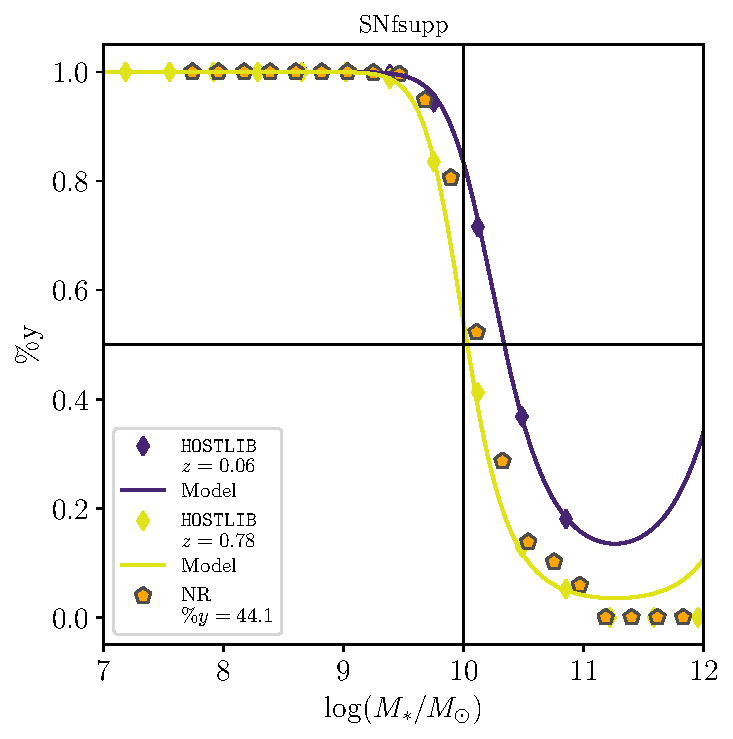
\includegraphics[width=.5\linewidth]{snana_diagnostic_fyvM_NRSNFSUPP}
    \caption[Fraction de jeunes étoiles en fonction de la masse pour le modèle
    de masse SNfsupp]{\textit{En violet (jaune)}~: fraction de jeunes étoiles en
        fonction de la masse pour le modèle de masse SNfsupp au redshift moyen
        de la \hostlib\ utilisée à hauts (bas) redshifts.\smallbreak \textit{En
        orange}~: même fraction mais pour l'échantillon simulé NR. Nous
        observons bien ici la suppression du modèle pour
    $M_* > 10^{11}\si{\Msun}$.}
    \label{fig:fyvMsupp}
\end{SCfigure}
\sidecaptionvpos{figure}{t}

Ensuite, pour avoir une comparaison efficace, nous effectuons une sélection
aléatoire des données de chaque sondage pour reproduire les ratios attendus. Les
quantités de données de ces mesures, exprimées en pourcentages de l'échantillon
Pantheon, sont égales aux ratios du plus petit sondage simulé des données non
échantillonnées~: ceux de la colonne «~SDSS~» du Tableau~\ref{tab:ratio}.

Nous rappelons que les modèles~\citetalias{popovic2021a}
et~\citetalias{scolnic2016} utilisent des distributions des paramètres
spécifiquement ajustés aux données~: BP utilisent des distributions gaussiennes
asymétriques, avec 3 paramètres libres, dans des intervalles de
\SI{0.2e10}{\Msun} (10 pour LOWZ, 20 pour les autres) pour reproduire
l'étirement des SNe~Ia~; SK incluent également des distributions gaussiennes
asymétriques, une pour chacun des sondages SDSS, PS1 et SNLS, et la distribution
donnée Équation~\ref{eq:sklowz} avec 6 paramètres libres, pour un total de $k =
15$. À l'inverse, les modélisations NN et NR reposent sur une modélisation
prospective, basée sur une modélisation de l'étirement avec 5 paramètres libres
ainsi qu'une modélisation de la masse avec 4 paramètres libres. L'évolution de
la fraction de jeunes étoiles repose sur 2 paramètres ($K$, $\Phi$) qui sont
fixés.

Nous nous intéressons dans un premier temps à l'ajustement en 1 dimension des
paramètres (Section~\ref{ssec:comp1d}) avant de traiter l'aspect bi-dimensionnel
(Section~\ref{ssec:comp2d}).

\subsection{Accord entre les données~: analyse uni-dimensionnelle}\label{ssec:comp1d}

Nous présentons ici les résultats des simulations de paramètres de redshift,
étirement et masse des différentes modélisations dont les représentations
graphiques sont données Figure~\ref{fig:hist1d}.

\begin{figure}[ht]
    \centering
    \includegraphics[width=.8\linewidth]{snana_diagnostic_hist_all-panth_only_allSNFSUPP}
    \caption[Histogrammes uni-dimensionnels des données simulées et réelles]
        {Histogrammes normés des données simulées (en lignes pleines
        colorées) et des données réelles (en gris) selon le modèle et le
        paramètre. \textit{De gauche à droite}~: résultats pour les modèles SK,
        BP, NN et NR, respectivement. \textit{De haut en bas}~: nombre de
        données simulées en fonction du redshift, de l'étirement et de la masse,
        respectivement. Les valeurs de $\chi^2$ entre les données simulées et
        réelles sont indiquées dans le coin supérieur droit de chaque figure, et
        de vert à rouge du plus petit au plus grand. Nous indiquons en points
        noirs le modèle d'étirement de~\citetalias{nicolas2021} au redshift
        moyen de l'échantillon Pantheon.}
    \label{fig:hist1d}
\end{figure}

Pour chacune des comparaisons, nous calculons une valeur de $\chi^2$. Pour cela,
nous normalisons les histogrammes des données simulées au nombre de données de
Pantheon, puis calculons~:
\begin{equation}\label{eq:chi21d}
    \chi^2 = \frac{1}{N}\times\sum_{i=0}^{N-1} \frac{(d_i - s_i)^2}{d_i+s_i}
\end{equation}
avec $N$ le nombre d'intervalles des histogrammes et $d_i$ ($s_i$) le nombre de
données réelles (simulées) dans l'intervalle $i$. Le meilleur accord est décrit
par le $\chi^2$ le plus petit. Les valeurs sont indiquées
Tableau~\ref{tab:chi21d}.

\newcommand{\ccg}{\cellcolor{limegreen!20}}
\newcommand{\ccr}{\cellcolor{red!10}}
\newcommand{\ccy}{\cellcolor{yellow!20}}
\newcommand{\cco}{\cellcolor{orange!20}}
\begin{table}[ht]
    \centering
        \caption[Comparaison de la capacité de chaque simulation à représenter
        les données en une dimension]{Valeurs de $\chi^2$ donnant la comparaison
            de la capacité de chaque simulation à représenter les données de
        redshift, d'étirement et de masse.}
        \label{tab:chi21d}
    \begin{threeparttable}
        \makebox[\linewidth]{%
        \begin{tabular}{lcccc}
            \toprule
                    & \multicolumn{4}{c}{$\chi^2$} \\ \cmidrule(lr){2-5}
            Paramètre & SK & BP & NN & NR \\
            \midrule
            Redshift    & \ccg\ 4.34  & \ccy\ 4.92  & \cco\ 5.36  & \ccr\ 6.26 \\
            Étirement   & \ccr\ 5.01  & \ccg\ 2.91  & \cco\ 4.01  & \ccy\ 3.83 \\
            Masse       & \ccr\ 4.97  & \cco\ 4.43  & \ccy\ 3.96  & \ccg\ 3.58 \\
            \midrule
            Somme       & \ccr\ 14.32 & \ccg\ 12.26 & \ccy\ 13.33 & \cco\ 13.67\\
            Probabilité & \ccr\ 0.36  & \ccg\ 1.00  & \ccy\ 0.59  & \cco\ 0.49 \\
            \bottomrule
    \end{tabular}}
        \begin{tablenotes}[flushleft]
            \item \small \textbf{\hspace{-3,2pt}Notes.} Pour chaque simulation,
                une sélection des données est réalisée pour correspondre aux
                ratios des données de Pantheon, et le calcul du $\chi^2$ est la
                moyenne sur 500 de ces tirages à chaque fois. La probabilité est
                donnés par rapport au meilleur modèle (BP), telle que
                $\mathcal{P}_{\text{modèle}} =
                \exp^{(\chi^2_{\rm BP} - \chi^2_{\text{modèle}})/2}$.
        \end{tablenotes}
    \end{threeparttable}
\end{table}

D'une manière globale, le modèle BP apparaît comme la meilleure description des
données, NN et NR donnent des résultats similaires et SK a le moins bon accord.
Pour le redshift cependant, c'est le modèle SK qui est le mieux ajusté aux
données. Ceci correspond à nos attentes puisque leurs distributions
d'étirements se divisent suivant le redshift. Pour la masse, étant donné que
toutes les simulations utilisent les mêmes \wgtmap, les différences sont moins
notables. NR donne cependant une meilleure représentation des données, mais pas
de manière significative. Pour l'étirement, c'est BP qui décrit le mieux les
données. Ceci correspond également à nos attentes puisque leurs distributions
d'étirements sont nombreuses. Nous notons cependant que pour ce paramètre, les
modèles NN et NR sont bien représentatifs des données. En regardant par
échantillon, nous observons qu'en réalité les modèles NN et NR performent en
moyenne bien mieux que les deux autres mais ont par contre une certaine
difficulté à reproduire la distribution de LOWZ. En effet, par la nature ciblée
du sondage, la prédiction du modèle de~\citetalias{nicolas2021} ne peut
s'appliquer, ce qui mène à leurs valeurs de $\chi^2$ que nous détaillons
Tableau~\ref{tab:chix1}. Nous présentons Figure~\ref{fig:lowz1d} l'accord entre
données simulées et réelles de l'échantillon LOWZ pour les différents modèles.

\begin{table}[ht]
    \centering
        \caption[Comparaison de la capacité de chaque simulation à représenter
        les données d'étirement selon le sondage]{Valeurs de $\chi^2$ donnant la
            comparaison de la capacité de chaque simulation à représenter les
        données d'étirement pour chaque sondage simulé.}
        \label{tab:chix1}
    \begin{threeparttable}
        \makebox[\linewidth]{%
        \begin{tabular}{lcccc}
            \toprule
                    & \multicolumn{4}{c}{$\chi^2$} \\ \cmidrule(lr){2-5}
            Sondage   & SK          & BP          & NN          & NR \\
            \midrule
            LOWZ      & \ccy\ 14.63 & \ccg\ 10.29 & \ccr\ 37.05 & \cco\ 36.84 \\
            SDSS      & \ccg\ 7.03  & \ccr\ 8.52  & \cco\ 7.66  & \ccy\ 7.05 \\
            PS1       & \ccr\ 10.35 & \ccg\ 3.58  & \ccy\ 4.06  & \cco\ 4.29 \\
            SNLS      & \cco\ 15.14 & \ccr\ 23.13 & \ccy\ 15.03 & \ccg\ 15.00 \\
            \midrule
            Somme     & \ccy\ 47.15 & \ccg\ 45.52 & \ccr\ 63.80 & \cco\ 63.18 \\
            Sans LOWZ & \ccr\ 35.52 & \cco\ 35.23 & \ccy\ 26.75 & \ccg\ 26.34 \\

            \bottomrule
    \end{tabular}}
        \begin{tablenotes}[flushleft]
            \item \small \textbf{\hspace{-3,2pt}Notes.} Ici, aucun tirage n'est
                réalisé.
        \end{tablenotes}
    \end{threeparttable}
\end{table}

\begin{figure}[ht]
    \centering
    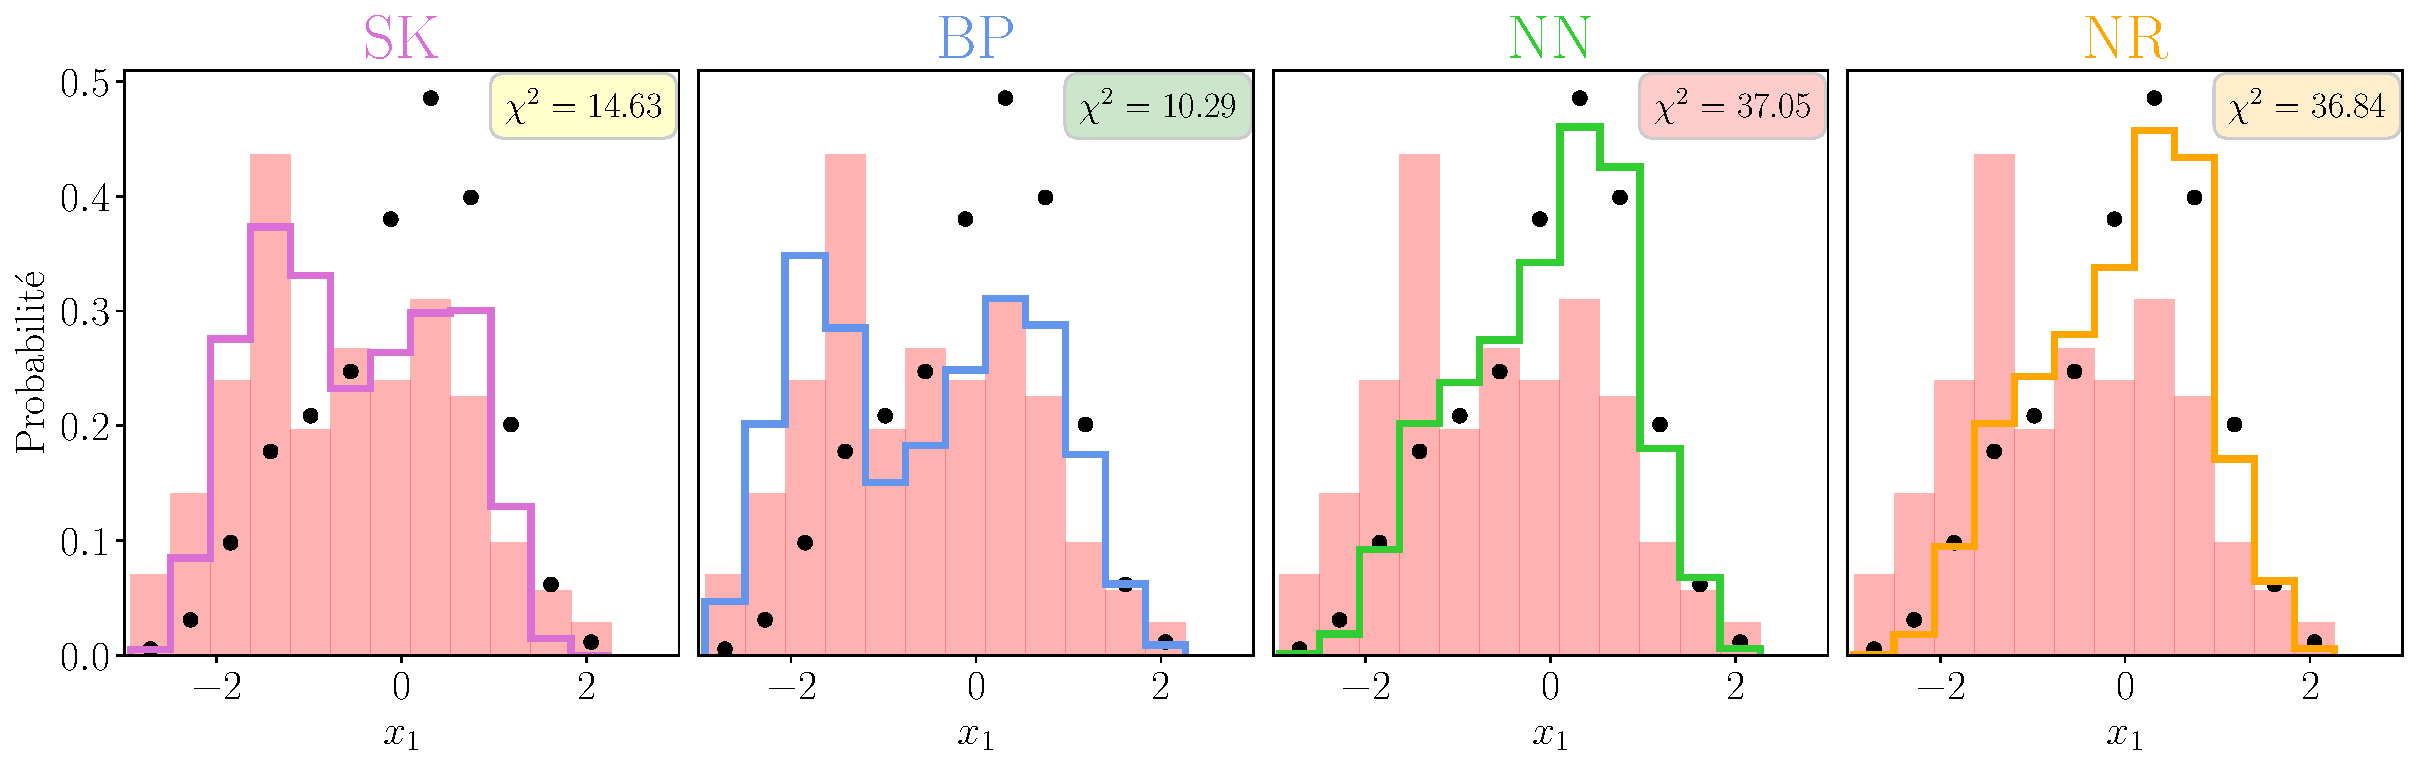
\includegraphics[width=\linewidth]{snana_diagnostic_hist_x1-panth_LOWZ_SNFSUPP}
    \caption[Histogrammes uni-dimensionnels des étirements des données simulées
    et réelles pour l'échantillon LOWZ]{Histogrammes normés des étirements des
        données simulées (en lignes pleines colorées) et des données réelles (en
        rouge) pour le sondage LOWZ selon le modèle. \textit{De gauche à
        droite}~: résultats pour les modèles SK, BP, NN et NR, respectivement.
        Les valeurs de $\chi^2$ entre les données simulées et réelles sont
        indiquées dans le coin supérieur droit de chaque figure, et de vert à
        rouge du plus petit au plus grand. Nous indiquons en points noirs le
        modèle d'étirement de~\citetalias{nicolas2021} au redshift moyen de
    l'échantillon LOWZ.}
    \label{fig:lowz1d}
\end{figure}

Il reste que dans la pratique, tous sondages confondus, les résultats des
différents modèles sont compatibles entre eux, et nous pouvons tous les
considérer comme de bonnes représentations des données. Pour LOWZ
spécifiquement, nous pourrions améliorer la simulation du sondage \textit{via}
la modification du modèle~\citetalias{nicolas2021} pour l'étirement, notamment
en incluant les données de ZTF (Section~\ref{ssec:zres}) ou en utilisant la
fraction de jeunes étoiles escomptée. En effet, le modèle d'évolution de la
fraction de jeunes étoiles $\delta(z)$ donne une valeur de 50\% de jeunes SNe~Ia
à $z = 0,05$. Or dans notre cas, le sondage se situe à un redshift moyen de $z =
0,03$ mais les données testées (voir Chapitre~\ref{ch:snana},
Figure~\ref{fig:snana_func}) du modèle NR n'en possèdent que 20\%, réduits à
15\% dans les données conservées. Comme nous avons créé notre \hostlib\ en
utilisant le redshift de chaque entrée, l'accord avec les données est de fait
erroné, et il est probable que la vraie fraction soit encore plus faible en
observant ces résultats Figure~\ref{fig:lowzdump}. Pour y remédier, nous
pourrions utiliser le modèle d'étirement Base+const\footnote{C'est le modèle de
base avec une fraction fixe de jeunes étoiles.} du Chapitre~\ref{ch:stretch} en
ajustant la fraction aux données de LOWZ, et utiliser ce modèle indépendamment
du redshift de la \hostlib.

\sidecaptionvpos{figure}{c}
\begin{SCfigure}[1][ht]
    \centering
    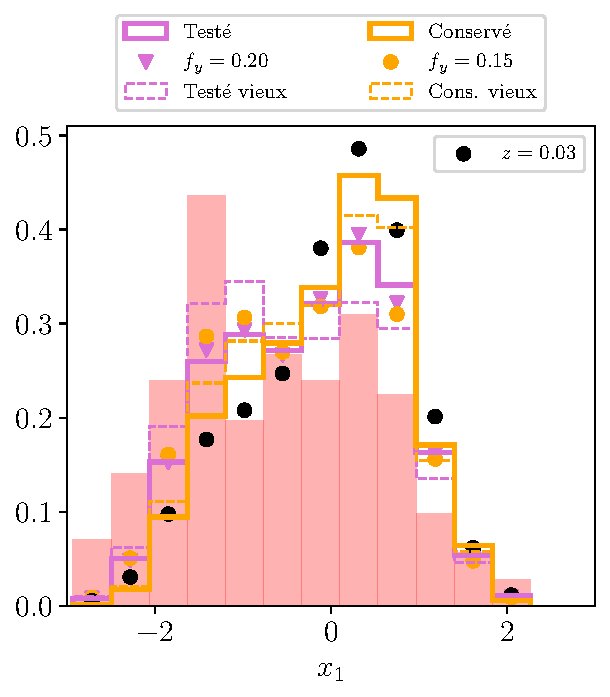
\includegraphics[width=.5\linewidth]{snana_diagnostic_hist_x1-panth_surv_NRSNFSUPP-LOWZ}
    \caption[Histogrammes des données testées et conservées du modèle NR pour le
    sondage LOWZ]{Histogrammes des étirements des données de LOWZ~:\textit{en
        rouge} celles de Pantheon~; \textit{en violet} les données testées et
        \textit{en orange} les données conservées pour le modèle NR. Le
        modèle~\citetalias{nicolas2021} évalué aux fractions des jeunes SNe~Ia
        pour ces deux échantillons sont tracés en marqueurs de la couleur
        correspondante~; le modèle évalué au redshift moyen de la distribution
        est tracé en marqueurs noirs. Les parties vieilles des données testées
    et conservées sont en pointillés.}
    \label{fig:lowzdump}
\end{SCfigure}
\sidecaptionvpos{figure}{t}

\subsection{Accord entre les données~: analyse
bi-dimensionnelle}\label{ssec:comp2d}

Nous présentons maintenant les distributions d'étirement en fonction du redshift
d'une part et les distributions d'étirement en fonction de la masse de la
galaxie hôte d'autre part. Pour déterminer l'accord entre les échantillons réels
et simulés de manière quantitative, nous avons utilisé une estimation par noyau
pour convertir les données simulées en densité de probabilité bi-dimensionnelle,
permettant de calculer une probabilité totale traduisant l'accord entre les
données réelles et le noyau. Deux exemples sont donnés Figure~\ref{fig:2dhex},
où nous représentons les distributions des données simulées \textit{via} son
estimation par noyau en couleurs et en points dispersés pour les données
réelles. Les résultats sont indiqués dans le Tableau~\ref{tab:chi2comp}~: une
plus grande probabilité représente un meilleur accord.

% \begin{figure}[ht]
%     \centering
%     \begin{subfigure}[]{.48\linewidth}
%         \centering
%         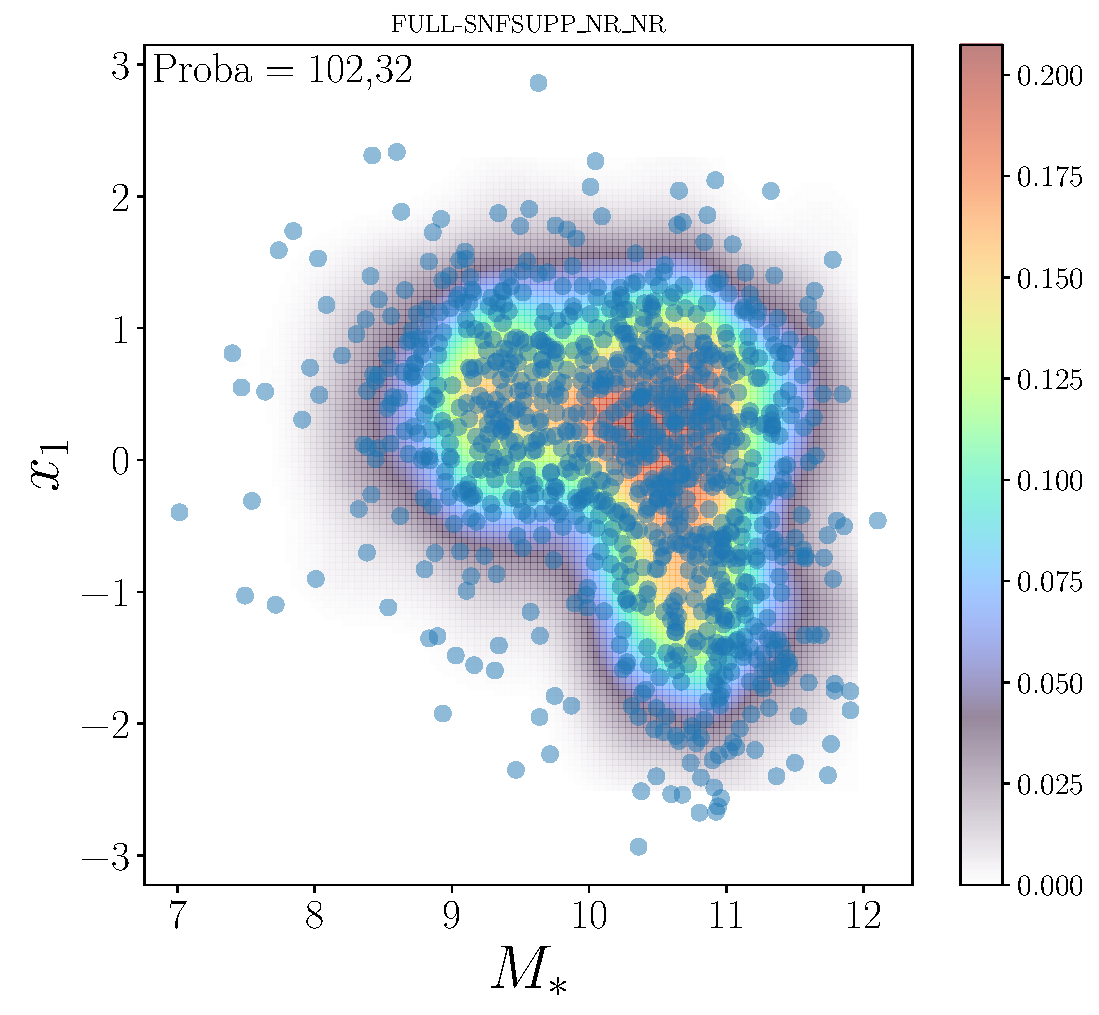
\includegraphics[width=\linewidth]{FULL-SNFSUPP_NR_NR_MS_kernel}
%         \caption[Accord entre données réelles et simulées pour les paramètres de
%         masse et d'étirement]{\footnotesize\textit{En abscisse}~: masse
%         ($> 10^7\si{\Msun}$).\\\hspace*{15.5pt}
%         \textit{En ordonnée}~: étirement.}
%         \label{fig:hexnrms}
%     \end{subfigure}
%     \hfill
%     \begin{subfigure}[]{.48\linewidth}
%         \centering
%         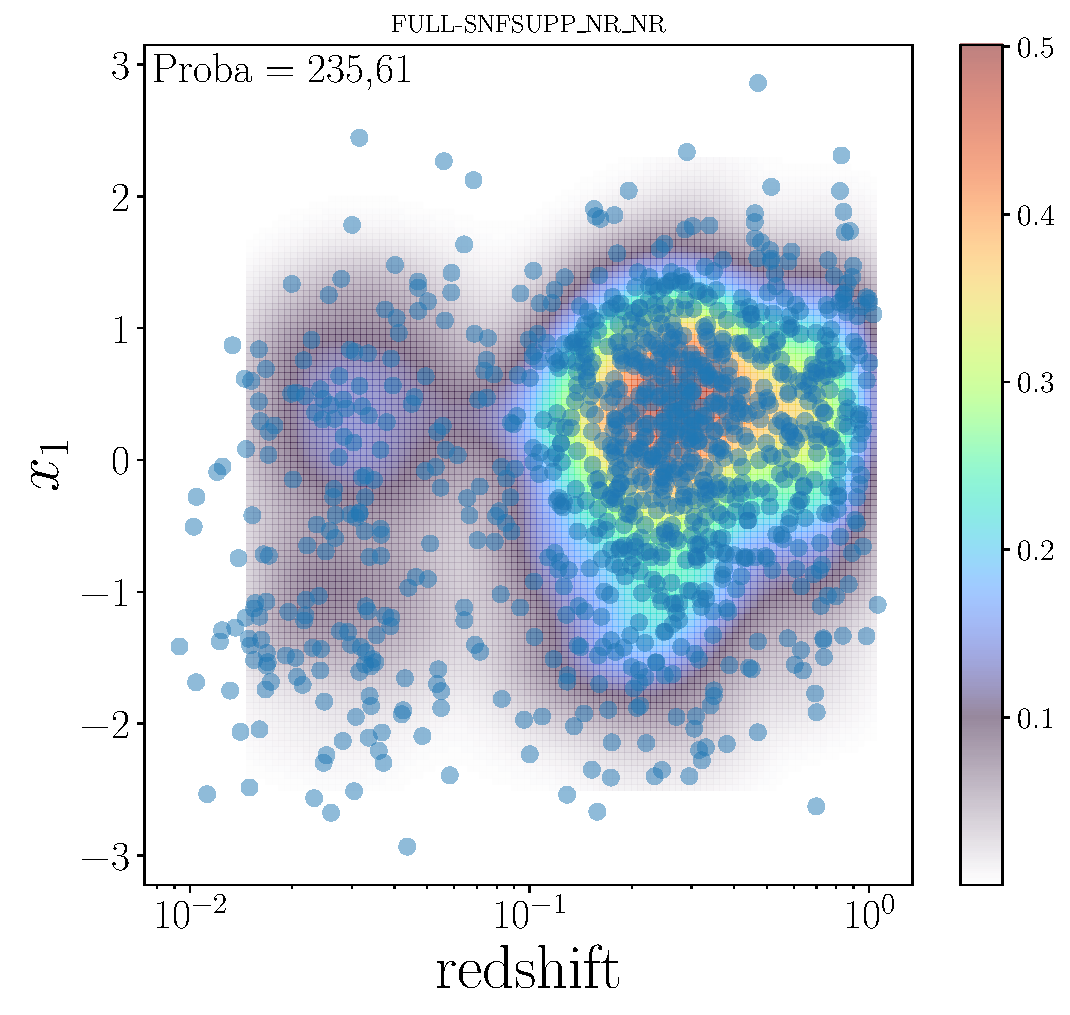
\includegraphics[width=\linewidth]{FULL-SNFSUPP_NR_NR_RS_kernel}
%         \caption[Accord entre données réelles et simulées pour les paramètres de
%         redshift et d'étirement]{\footnotesize\textit{En abscisse}~: redshift
%         (logarithmique).\\\hspace*{15.5pt}
%     \textit{En ordonnée}~: étirement.}
%         \label{fig:hexnrrs}
%     \end{subfigure}
%     \caption[Accord entre les données réelles et simulées pour le modèle
%     NR]{Accord entre les données réelles et simulées pour le modèle NR.
%         L'estimation par noyau donnant la densité de probabilité est indiquée en
%         couleur (voir la barre de couleur). L'accord est indiqué sous la forme
%     d'une probabilité en haut à gauche.}
%     \label{fig:2dhex}
% \end{figure}

\begin{figure}[p]
    \vspace*{-2.2cm}
    \thisfloatpagestyle{empty}
    \centerfloat
    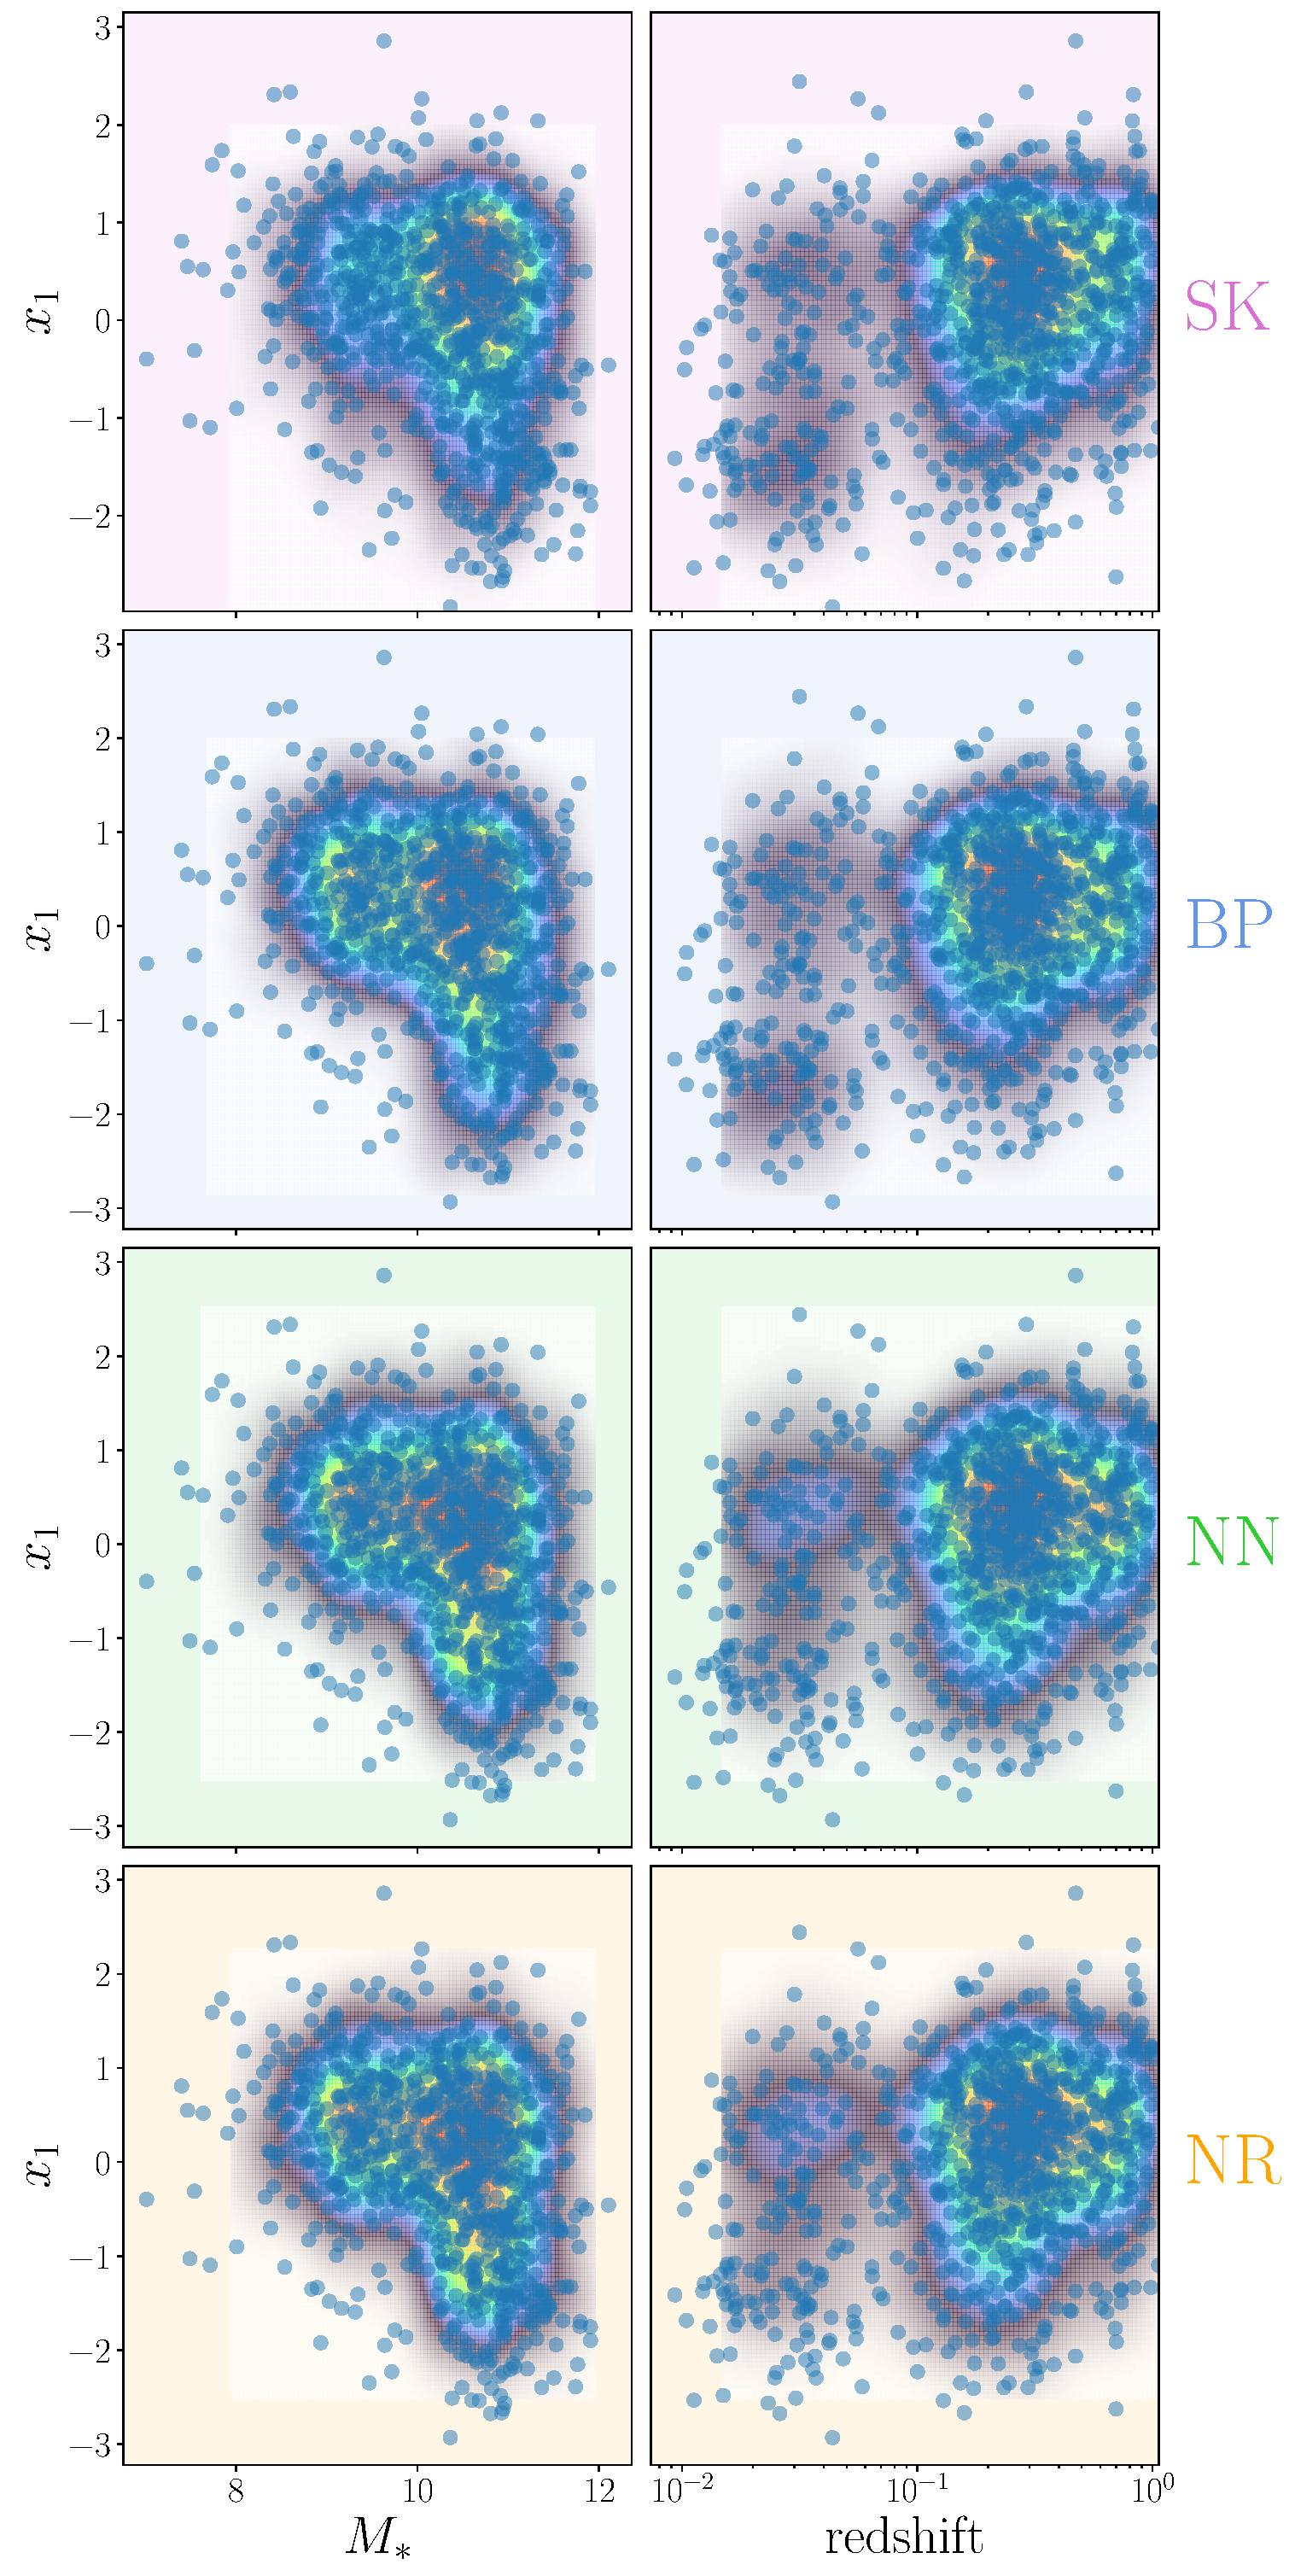
\includegraphics[width=.9\linewidth]{FULL-SNFSUPP_all_RS-MS_kernels}
    \caption[Accord entre les données réelles et simulées en 2 dimensions pour
    tous les modèles]{Accord données réelles (en points bleus transparents) et
        simulées (en couleur) en 2D pour tous les modèles. \textit{À gauche}~:
        étirement en ordonnée et masse en abscisse. \textit{À droite}~:
        étirement en ordonnée et redshift en abscisse. \textit{De haut en bas}~:
    modèles SK, BP, NN et NR, respectivement, voir légende. Les couleurs
correspondent à celles de la Figure~\ref{fig:hist1d}.}
    \label{fig:2dhex}
\end{figure}

\begin{table}[ht]
    \centering
     \caption[Comparaison de la capacité de chaque simulation à représenter
        les données en deux dimensions]{Comparaison de la capacité de chaque
            simulation à représenter les données d'étirement et de masse d'une
        part, et d'étirement et de redshift d'autre part.}
    \label{tab:chi2comp}
    \begin{threeparttable}
    \makebox[\linewidth]{%
    \begin{tabular}{lccc}
        \toprule
                & \multicolumn{3}{c}{Probabilité} \\ \cmidrule(lr){2-4}
        Modèles & $x_1$ vs $M_*$ & $x_1$ vs $z$ & Somme \\
        \midrule
        \ccg\ SK & \ccy\ 103,03 & \ccg\ 252,57 & \ccg\ 355,60 \\
        \ccy\ BP & \ccg\ 103,37 & \ccy\ 246,49 & \ccy\ 349,85 \\
        \cco\ NN & \cco\ 102,35 & \cco\ 236,25 & \cco\ 338,60 \\
        \ccr\ NR & \ccr\ 102,32 & \ccr\ 235,61 & \ccr\ 338,93 \\
        \bottomrule
    \end{tabular}}
    \begin{tablenotes}[flushleft]
        \item \small \textbf{\hspace{-3,2pt}Notes.} Pour chaque simulation, nous
            calculons une estimation par noyau bi-dimensionnelle sur les données
            simulées et nous l'utilisons pour déterminer chaque probabilité.
    \end{tablenotes}
    \end{threeparttable}
\end{table}

Nous observons que la modélisation~\citetalias{scolnic2016} est la meilleure des
quatre sur la combinaison de ces distributions~; la
modélisation~\citetalias{popovic2021a} est deuxième, et les
modélisations~\citetalias{nicolas2021} et NR ont un score similaire, les plaçant
comme les modélisations les moins bien ajustées aux données. C'est attendu étant
donné la différence du nombre de paramètres libres. Les résultats ne diffèrent
que très peu sur les distributions conjointes de redshift et de masse, et la
majeure partie de la différence entre les modèles vient de la modélisation
conjointe de l'étirement et du redshift pour laquelle les valeurs de
probabilités varient plus rapidement du fait de la faible étendue des données
(voir barres de couleur). Nous observons cependant que les modèles SK et BP
présentent deux nuages de probabilités à peu près équivalents à $z < 0,1$,
correspondant au sondage LOWZ. À l'inverse pour NN et NR, le nuage de point de
haut étirement est plus prononcé que celui de petit étirement. Ceci découle
naturellement de la différence de modélisation de l'étirement de ce sondage,
comme discuté précédemment. Nous notons cependant que les quatre modèles donnent
un accord similaire aux données réelles.

\section{Impact sur la cosmologie}\label{sec:simres}

Maintenant que nous avons observé l'accord de chacun des modèles aux données
réelles, nous pouvons étudier le biais cosmologique causé par un traitement de
données ayant leur propre physique avec une correction potentiellement
différente. Pour cela, comme introduit Section~\ref{ssec:snaimpl}, nous
appliquons la méthode BBC7D \citep[][voir
Section~\ref{ssec:bbc7D}]{popovic2021a} sur les données des différents modèles
avec chacun des échantillons de BiasCor. Nous obtenons ainsi 16 échantillons
corrigés de taille $\approx \num{13000}$ (dont le nombre de données est indiqué
Tableau~\ref{tab:ratio}), chacun ayant une valeur de $w$, $\gamma_{\rm masse}$,
$\alpha$ et $\beta$. Pour rappel, nous avons fixé $\Omega_M$ à
$\num{0.315}\pm\num{0.005}$~; nous ne nous intéressons donc pas à la variation
de ce paramètre.

Nous présentons Section~\ref{ssec:simabg} les résultats pour les paramètres de
standardisation $\alpha$, $\beta$ et $\gamma$, nécessaires pour pouvoir comparer
les résultats sur le paramètre d'état de l'énergie noire $w$ dont les résultats
sont présentés Section~\ref{ssec:simw}. Nous discutons de l'impact du choix de
modèle de masse Section~\ref{ssec:modsys}.

\subsection{Résultats de standardisation}\label{ssec:simabg}

Afin d'avoir des résultats cosmologiques significatifs, nous nous sommes
intéressæ aux valeurs des paramètres $\alpha$, $\beta$ et $\gamma$ ajustées de
nos simulations.  Les résultats pour $\alpha$ sont indiqués sur la
Figure~\ref{fig:cosmo1}, et ceux de $\beta$ et $\gamma$ sont indiqués
Figure~\ref{fig:cosmo2}. Les couleurs représentent l'écart aux valeurs de
référence, avec $\gamma_{\rm ref} = \num{0.05}$. Nous nous attendons à ce que
les échantillons diagonaux ne présentent pas de biais de mesure, étant donné que
leur correction des données est cohérente avec leur génération.

\begin{figure}[ht]
    \centering
    \begin{subfigure}[]{.48\linewidth}
        \centering
        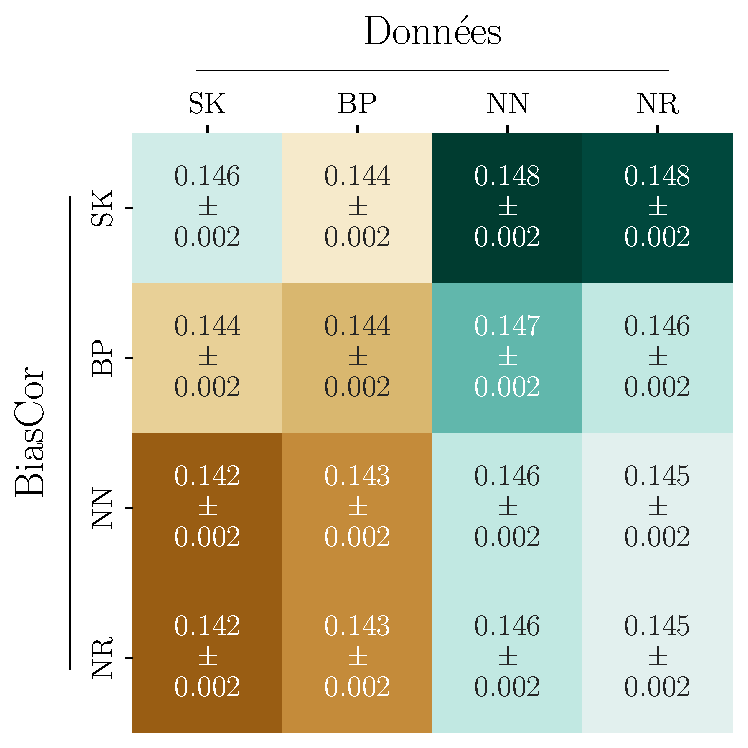
\includegraphics[width=\linewidth]{alphafit_covmat_FULL-SNFSUPP_2}
        \caption[Valeurs de $\alpha$ avec le modèle de masse SNfsupp]{Valeurs de
        $\alpha$.}
        \label{fig:cosmoa}
    \end{subfigure}
    \hfill
    \begin{subfigure}[]{.48\linewidth}
        \centering
        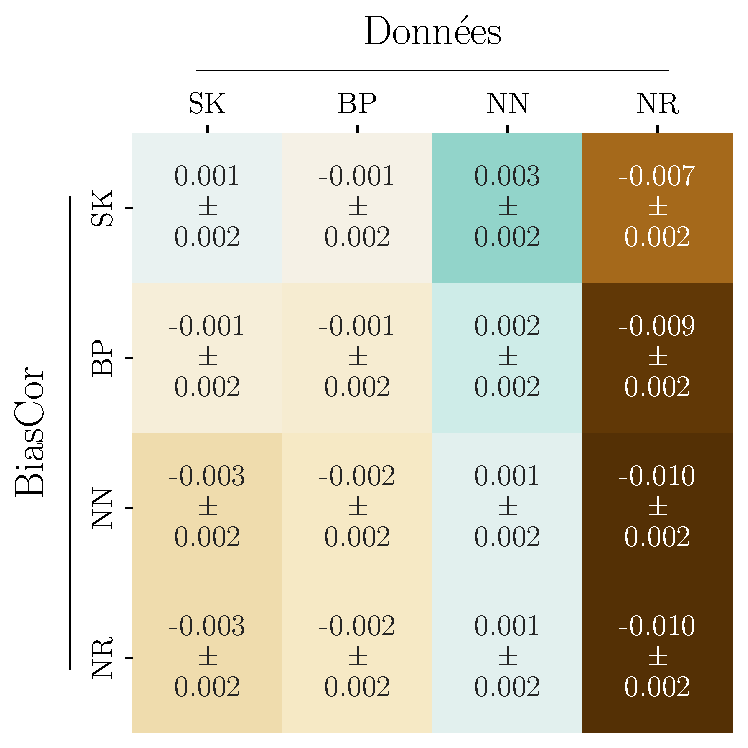
\includegraphics[width=\linewidth]{alphafit_covmat_FULL-SNFSUPP_2-bias}
        \caption[Valeurs de $\Delta\alpha$ avec le modèle de masse
        SNfsupp]{Valeurs de $\Delta\alpha$.}
        \label{fig:cosmoda}
    \end{subfigure}
    \caption[Résultats cosmologiques~: $\alpha$ et $\Delta\alpha$]{Résultats
        cosmologiques~: valeurs de $\alpha$ et $\Delta\alpha$ déterminées par
        ajustement avec la méthode BBC7D (voir
        Chapitre~\ref{ch:snana}). La figure de droite met en
        évidence que le modèle NR perçoit une valeur de référence de $\alpha =
    0,155$ au lieu de \num{0.145}.}
    \label{fig:cosmo1}
\end{figure}

\begin{figure}[h!]
    \centering
    \begin{subfigure}[]{.48\linewidth}
        \centering
        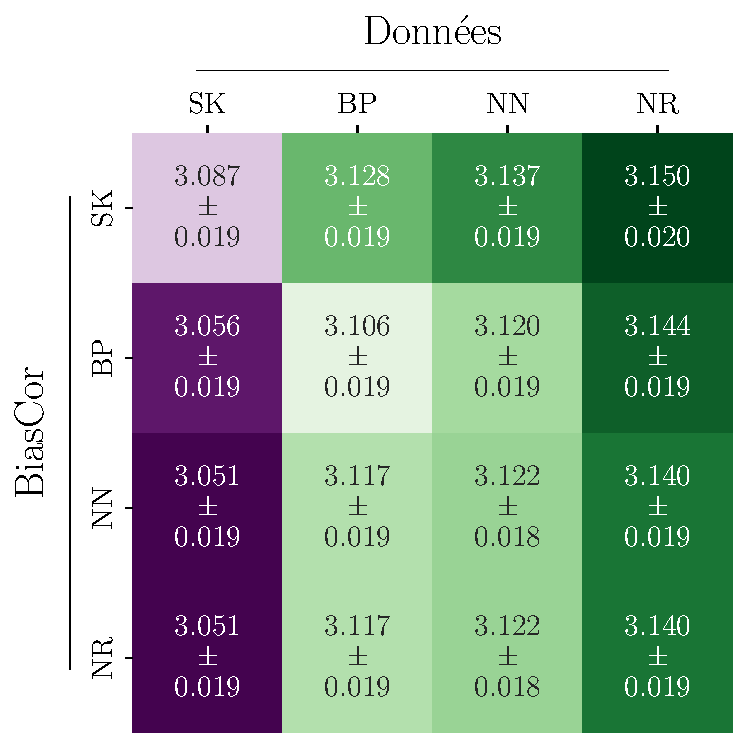
\includegraphics[width=\linewidth]{betafit_covmat_FULL-SNFSUPP_2}
        \caption[Valeurs de $\beta$ avec le modèle de masse SNfsupp]{Valeurs de
        $\beta$.}
        \label{fig:cosmob}
    \end{subfigure}
    \hfill
    \begin{subfigure}[]{.48\linewidth}
        \centering
        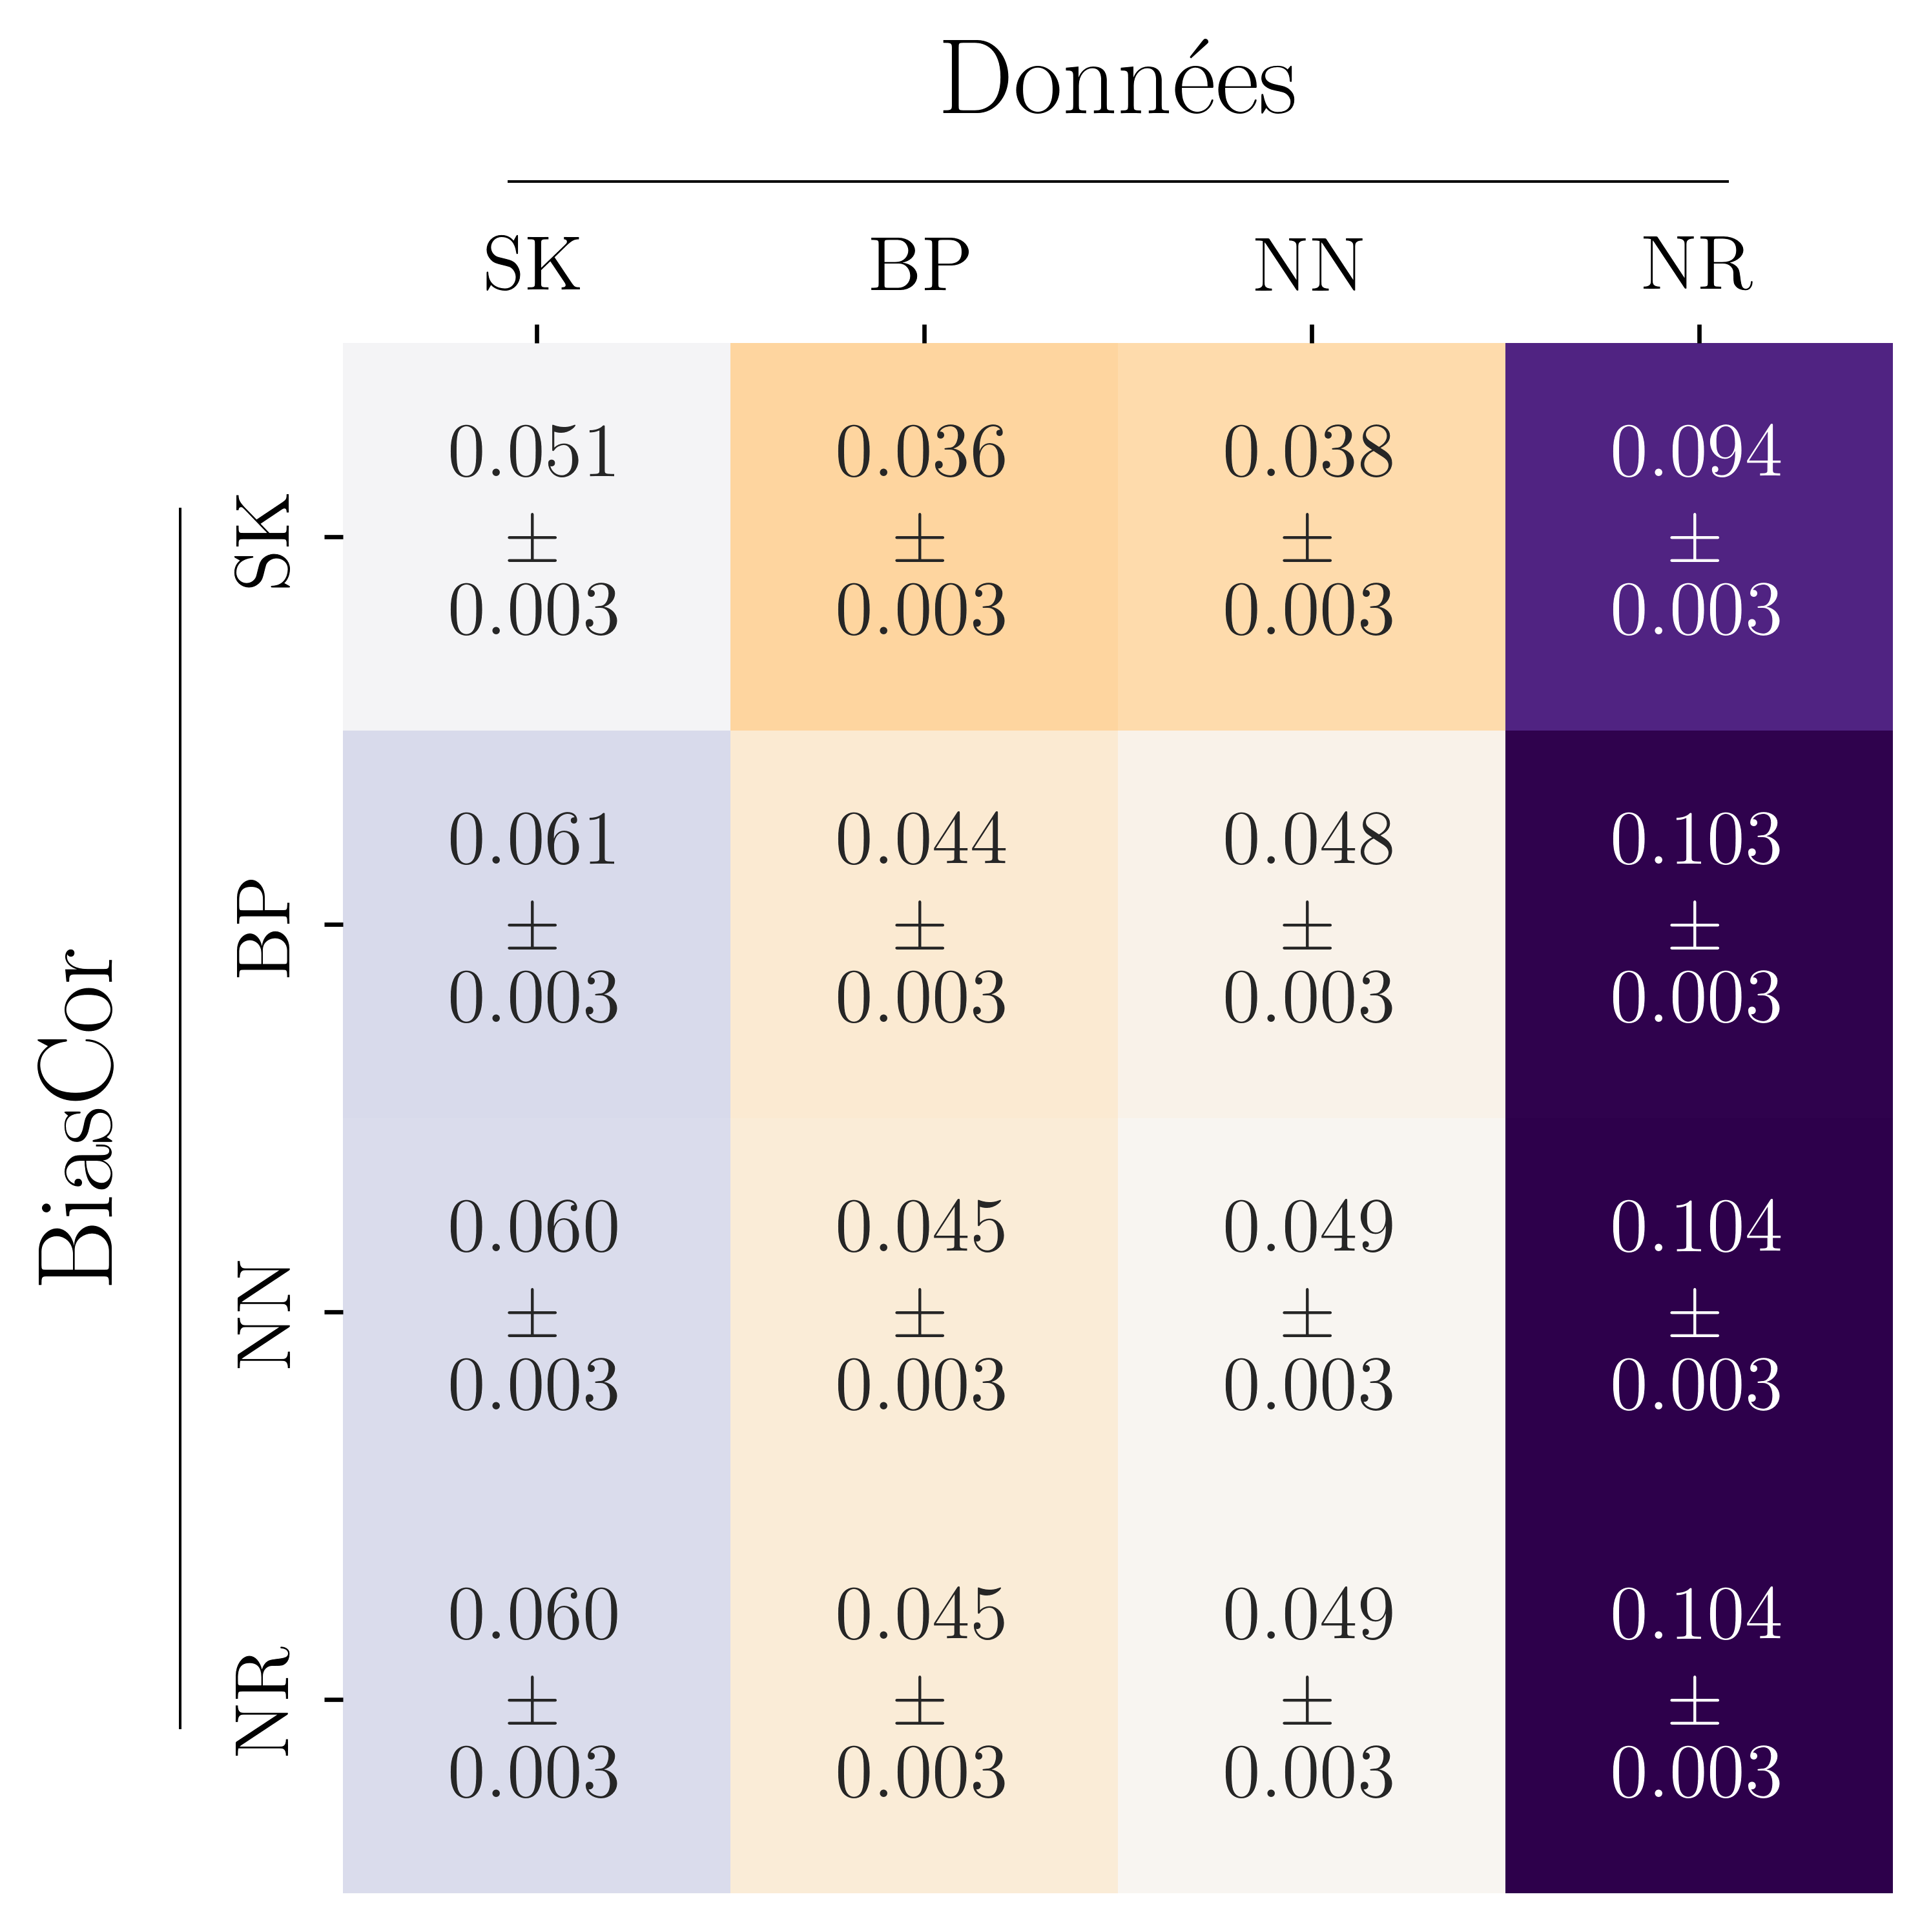
\includegraphics[width=\linewidth]{gammafit_covmat_FULL-SNFSUPP_2}
        \caption[Valeurs de $\gamma$ avec le modèle de masse SNfsupp]{Valeurs de
        $\gamma$.}
        \label{fig:cosmog}
    \end{subfigure}
    \caption[Résultats cosmologiques~: $\beta$ et $\gamma$]{Résultats
        cosmologiques~: valeurs de $\beta$ et $\gamma$ déterminées par ajustement
        avec la méthode BBC7D (voir
    Chapitre~\ref{ch:snana}).}
    \label{fig:cosmo2}
\end{figure}

Nous relevons que les deux dernières lignes présentent les mêmes valeurs. Cela
provient du fait que le procédé \bbc7D ne prend pas en compte la variation de
magnitude du modèle NR quand l'échantillon est utilisé comme BiasCor, puisqu'il
est évalué en tant que $\theta$ pour les données.

Afin de reproduire les résultats de l'analyse de Pantheon \citep{scolnic2018},
nous voulons que les valeurs de sorties des termes diagonaux soient compatibles
avec les valeurs d'entrées, $\alpha_{\rm ref} = \num{0.145}$ et $\beta_{\rm ref}
= \num{3.1}$. Lors de nos premières simulations, NR donnait une valeur de
$\alpha$ réduite à $\approx \num{0.135}$. Nous avons dû rehausser la valeur
d'entrée pour ce modèle à $\alpha_{\rm ref, NR} = \num{0.155}$ afin d'obtenir
une valeur satisfaisante. Ce biais est montré \textit{via} l'utilisation de
$\Delta\alpha = \alpha - \alpha_{\rm ref}$ sur la Figure~\ref{fig:cosmoda}. Nous
n'avons cependant pas ajusté la valeur $\beta$ de référence pour NR, bien
qu'elles soient $\approx 2\sigma$ écartées de la valeur de référence, puisque la
couleur n'est pas un paramètre que nous modifions dans la \hostlib\ NR~:
celle-ci utilise en effet les paramètres de BP, et nous avançons que le biais
sur $\beta$ est dû à un effet subtil reliant la couleur à l'étirement.

Sur l'ensemble de ces figures, nous voyons que les modèles SK, BP et NN sont
consistants avec eux-mêmes puisque les valeurs de sorties sont compatibles avec
la valeur d'entrée. S'il n'y a pas tant d'écart à \num{0.145} pour $\alpha$ dans
les termes non-diagonaux, nous notons que le modèle SK (pour lequel il n'existe
pas de corrélation entre galaxie et étirement/couleur) utilisé en tant que
données (colonne de gauche) présente des valeurs réduites quand il est corrigé
par les autres modèles (qui, eux, supposent des corrélations)~;  les valeurs
sont augmentées quand SK est utilisé comme BiasCor (ligne du haut). Ce même
résultat se retrouve pour les valeurs de $\beta$ (Figure~\ref{fig:cosmob}),
mais ce phénomène est inversé pour les valeurs de $\gamma$
(Figure~\ref{fig:cosmog})~: la colonne de gauche présente des valeurs plus
hautes et la ligne du haut des valeurs plus basses. Ces effets sont corrélés
puisque l'absence de corrélation entre galaxie et étirement/couleur du modèle SK
est compensé dans la valeur de marche de magnitude.

Pour NR, nous supposons que nous devons modifier la valeur de $\alpha_{\rm ref}$
en réponse à une mauvaise interprétation de la corrélation de la magnitude avec
l'âge par \snana. Le programme corrige cette magnitude \textit{via} la valeur de
la masse de la galaxie hôte et ne possède pas toute l'information nécessaire
pour comprendre cette corrélation. Ceci se répercute sur les résultats de
$\gamma_{\rm masse}$. En effet, alors que sa valeur d'entrée de marche de
magnitude basée sur l'âge est de \SI{0.130}{mag}, l'échantillon NR en tant que
données (colonne de droite, Figure~\ref{fig:cosmog}) donne des valeurs de marche
de magnitude basées sur la masse et ajustées par la méthode \bbc7D de
$\gamma_{\rm masse} \approx \num{.100}$, soit deux fois plus élevée que les
valeurs trouvées pour les autres simulations (de valeur d'entrée
\SI{0.05}{mag}).

\begin{figure}[t]
    \centering
    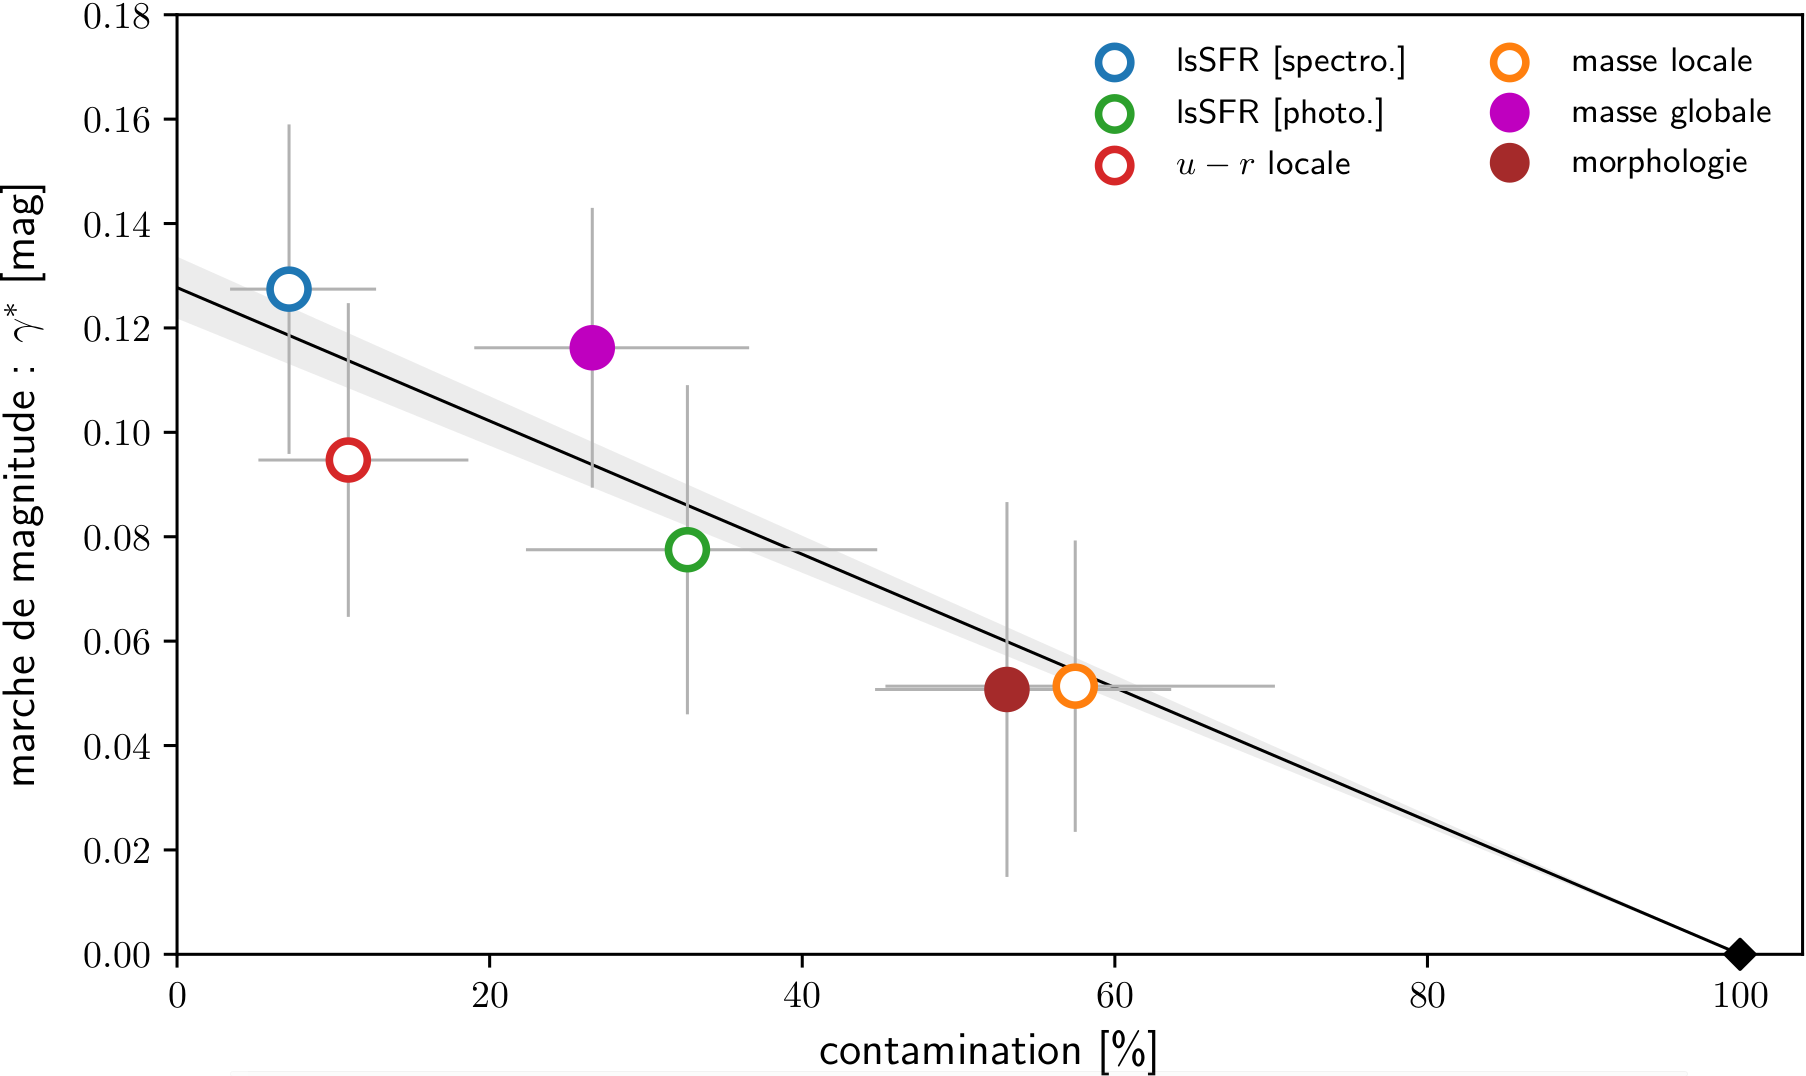
\includegraphics[width=.8\linewidth]{briday_steps-few}
    \caption[Marche de magnitude des SNe~Ia en fonction du traceur]{Marche de
        magnitude des SNe~Ia en fonction du traceur. Figure
        de~\cite{briday2021}. Les valeurs des marches de magnitude (points
        ouverts pour les traceurs locaux et pleins pour les globaux) sont
        déterminées sur l'échantillon SNf. Selon la capacité des traceurs à
        distinguer les populations de SNe~Ia (traduite par leur contamination),
        la marche de magnitude trouvée varie linéairement suivant la droite
        noire (avec son erreur en bande grise). En prenant le LsSFR comme
        traceur de référence avec $\gamma = \SI{0.13}{mag}$, la masse globale
        donnerait une marche de magnitude autour de \SI{0.10}{mag} sur cette
    ligne.}\label{fig:briday_steps}
\end{figure}

Cette déviation est attendue étant donné que la masse constitue un mauvais
traceur de l'âge d'une SN. Il est cependant intéressant de voir ces valeurs plus
basses que celle d'entrée~: c'est d'une part cohérent avec le fait que la
simulation voie un $\alpha_{\rm ref} = \num{0.155}$ (la baisse de $\gamma$ est
compensée dans $\alpha$, comme pour SK en tant que BiasCor), et d'autre part ce
résultat est en total accord avec l'étude de~\cite{briday2021}\footnote{Publiée
en anglais dans~\cite{briday2022}.}. L'auteur rapporte dans cet article qu'un
traceur moins efficace à différencier les populations de SNe~Ia attribuera une
marche de magnitude plus faible qu'un traceur plus discriminant. Notamment,
dans sa figure 8.1 (recopiée Figure~\ref{fig:briday_steps}), une valeur de
$\gamma = \SI{0.13}{mag}$ avec le LsSFR se traduirait par une valeur de $\gamma
\approx \SI{0.10}{mag}$ avec la masse globale (sur la ligne noire sous la masse
globale). Notre résultat est donc une confirmation de cet effet, réalisé de
manière complètement indépendante avec des données et des méthodes différentes,
ce qui vient conforter l'hypothèse que l'âge pourrait être le traceur des
propriétés intrinsèques des SNe~Ia.

\subsection{Résultats de cosmologie}\label{ssec:simw}

Dans la section précédente, nous nous sommes intéressæ aux corrélations
intrinsèques aux SNe~Ia impactant les paramètres de standardisation. Dans cette
section, nous présentons les résultats des valeurs de $w$ ajustées par \wfit\
(voir Section~\ref{ssec:bbcintro}) avec une valeur fixée de $\Omega_M =
\num{0.315}$. Ce sont des évolutions avec le redshift (erronées ou non) qui
impactent la valeur de $w$. Ainsi, nous présentons Figure~\ref{fig:wfit} les
résultats des valeurs ajustées de $w$, où les couleurs représentent l'écart à la
valeur de référence ($w = \num{-1.00}$), et pour comprendre ces résultats, nous
avons observé les évolutions des résidus de \textsc{Hubble} (voir
Chapitre~\ref{ch:snana}) en fonction du redshift pour chaque échantillon,
représentées Figure~\ref{fig:hr}. De même que précédemment, nous nous attendons
à ce que les termes diagonaux soient compatibles avec \num{-1.00}, et à ce que
les deux dernières lignes des figures soient similaires puisque les modèles NN
et NR forment les mêmes BiasCor.

\begin{figure}[ht]
    \centering
    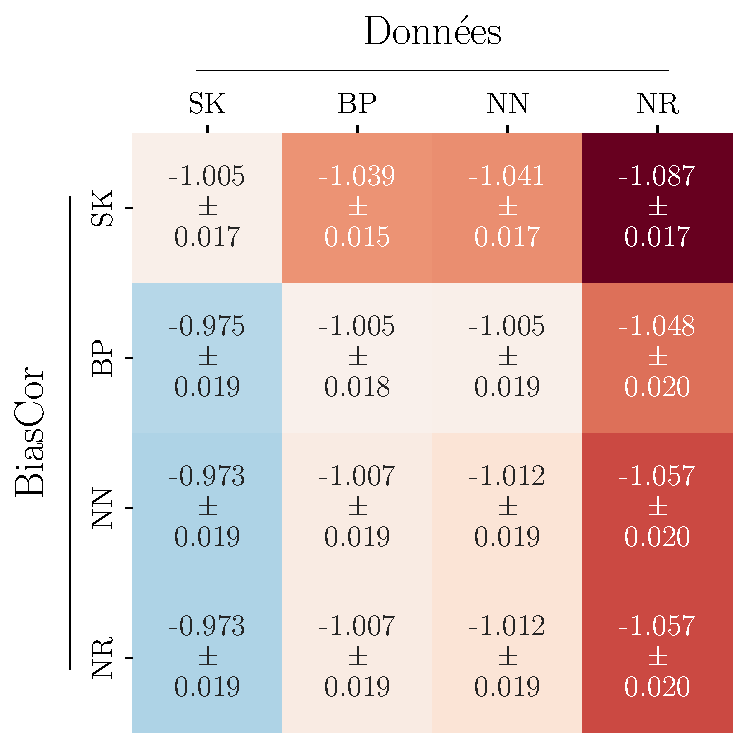
\includegraphics[width=.5\linewidth]{wfit_covmat_FULL-SNFSUPP_2}
    \caption[Résultats cosmologiques~: $w$]{Valeurs de $w$ déterminées par
    ajustement avec la méthode BBC7D (voir Chapitre~\ref{ch:snana}).}
    \label{fig:wfit}
\end{figure}

\begin{figure}[p]
    \centering
    \includegraphics[width=\linewidth]{HR_covmat-FULL-SNFSUPP_2}
    \caption[Résultats cosmologiques~: résidus de \textsc{Hubble}]{Résultats
        cosmologiques~: résidus de \textsc{Hubble} déterminés par ajustement
    avec la méthode BBC7D (voir Chapitre~\ref{ch:snana}).}
    \label{fig:hr}
\end{figure}

Pour rappel\footnote{Voir Chapitre~\ref{ch:cosmo}.}, nous définissons $w$, le
paramètre d'état de l'énergie sombre, \textit{via} l'équation mathématique
reliant la pression du fluide parfait la décrivant à sa densité d'énergie ($w =
p/\rho c^2$). Nous avions obtenu l'évolution de cette dernière en fonction du
facteur d'échelle $a$ de l'Univers suivant l'équation~\ref{eq:rho}~:
\begin{equation}
    \rho(t) \propto a(t)^{-3(1+w)}
\end{equation}
pour laquelle $w = -1$ donne une valeur de la pression constante dans le temps,
alors qu'une valeur de $w$ plus grande que \num{-1.00} (par exemple,
\num{-0.95}) impliquerait que l'effet de l'énergie sombre diminue avec le temps
($\rho(t)$ de la forme $\rho(t) \propto a(t)^{-x}$ avec $x > 0$) et une valeur
plus petite en augmenterait la puissance ($\rho(t) \propto a(t)^{+x}$ avec $x >
0$). Autrement dit, si $w > -1$, alors l'énergie sombre était plus puissante
dans le passé et le sera moins dans le futur. L'Univers serait donc en réalité
plus jeune que ce que nous croyons, et inversement. Ceci est illustré
Figure~\ref{fig:wevol}. Les données actuelles de Pantheon \citep{scolnic2018}
contraignent $w$ à $\pm \num{0.220}$ à elles seules, et à $\pm \num{0.040}$ avec
d'autres sondes, donnant des résultats compatibles avec \num{-1.00}. Les futurs
relevés visent quant à eux une détermination à $\pm \num{0.020}$, ce qui
pourrait mettre en évidence un décalage à $w = \num{-1.00}$. À cet effet, nos
simulations sont représentatives de ce qui pourra être atteint dans un futur
proche.

\sidecaptionvpos{figure}{c}
\begin{SCfigure}[1]
    \centering
    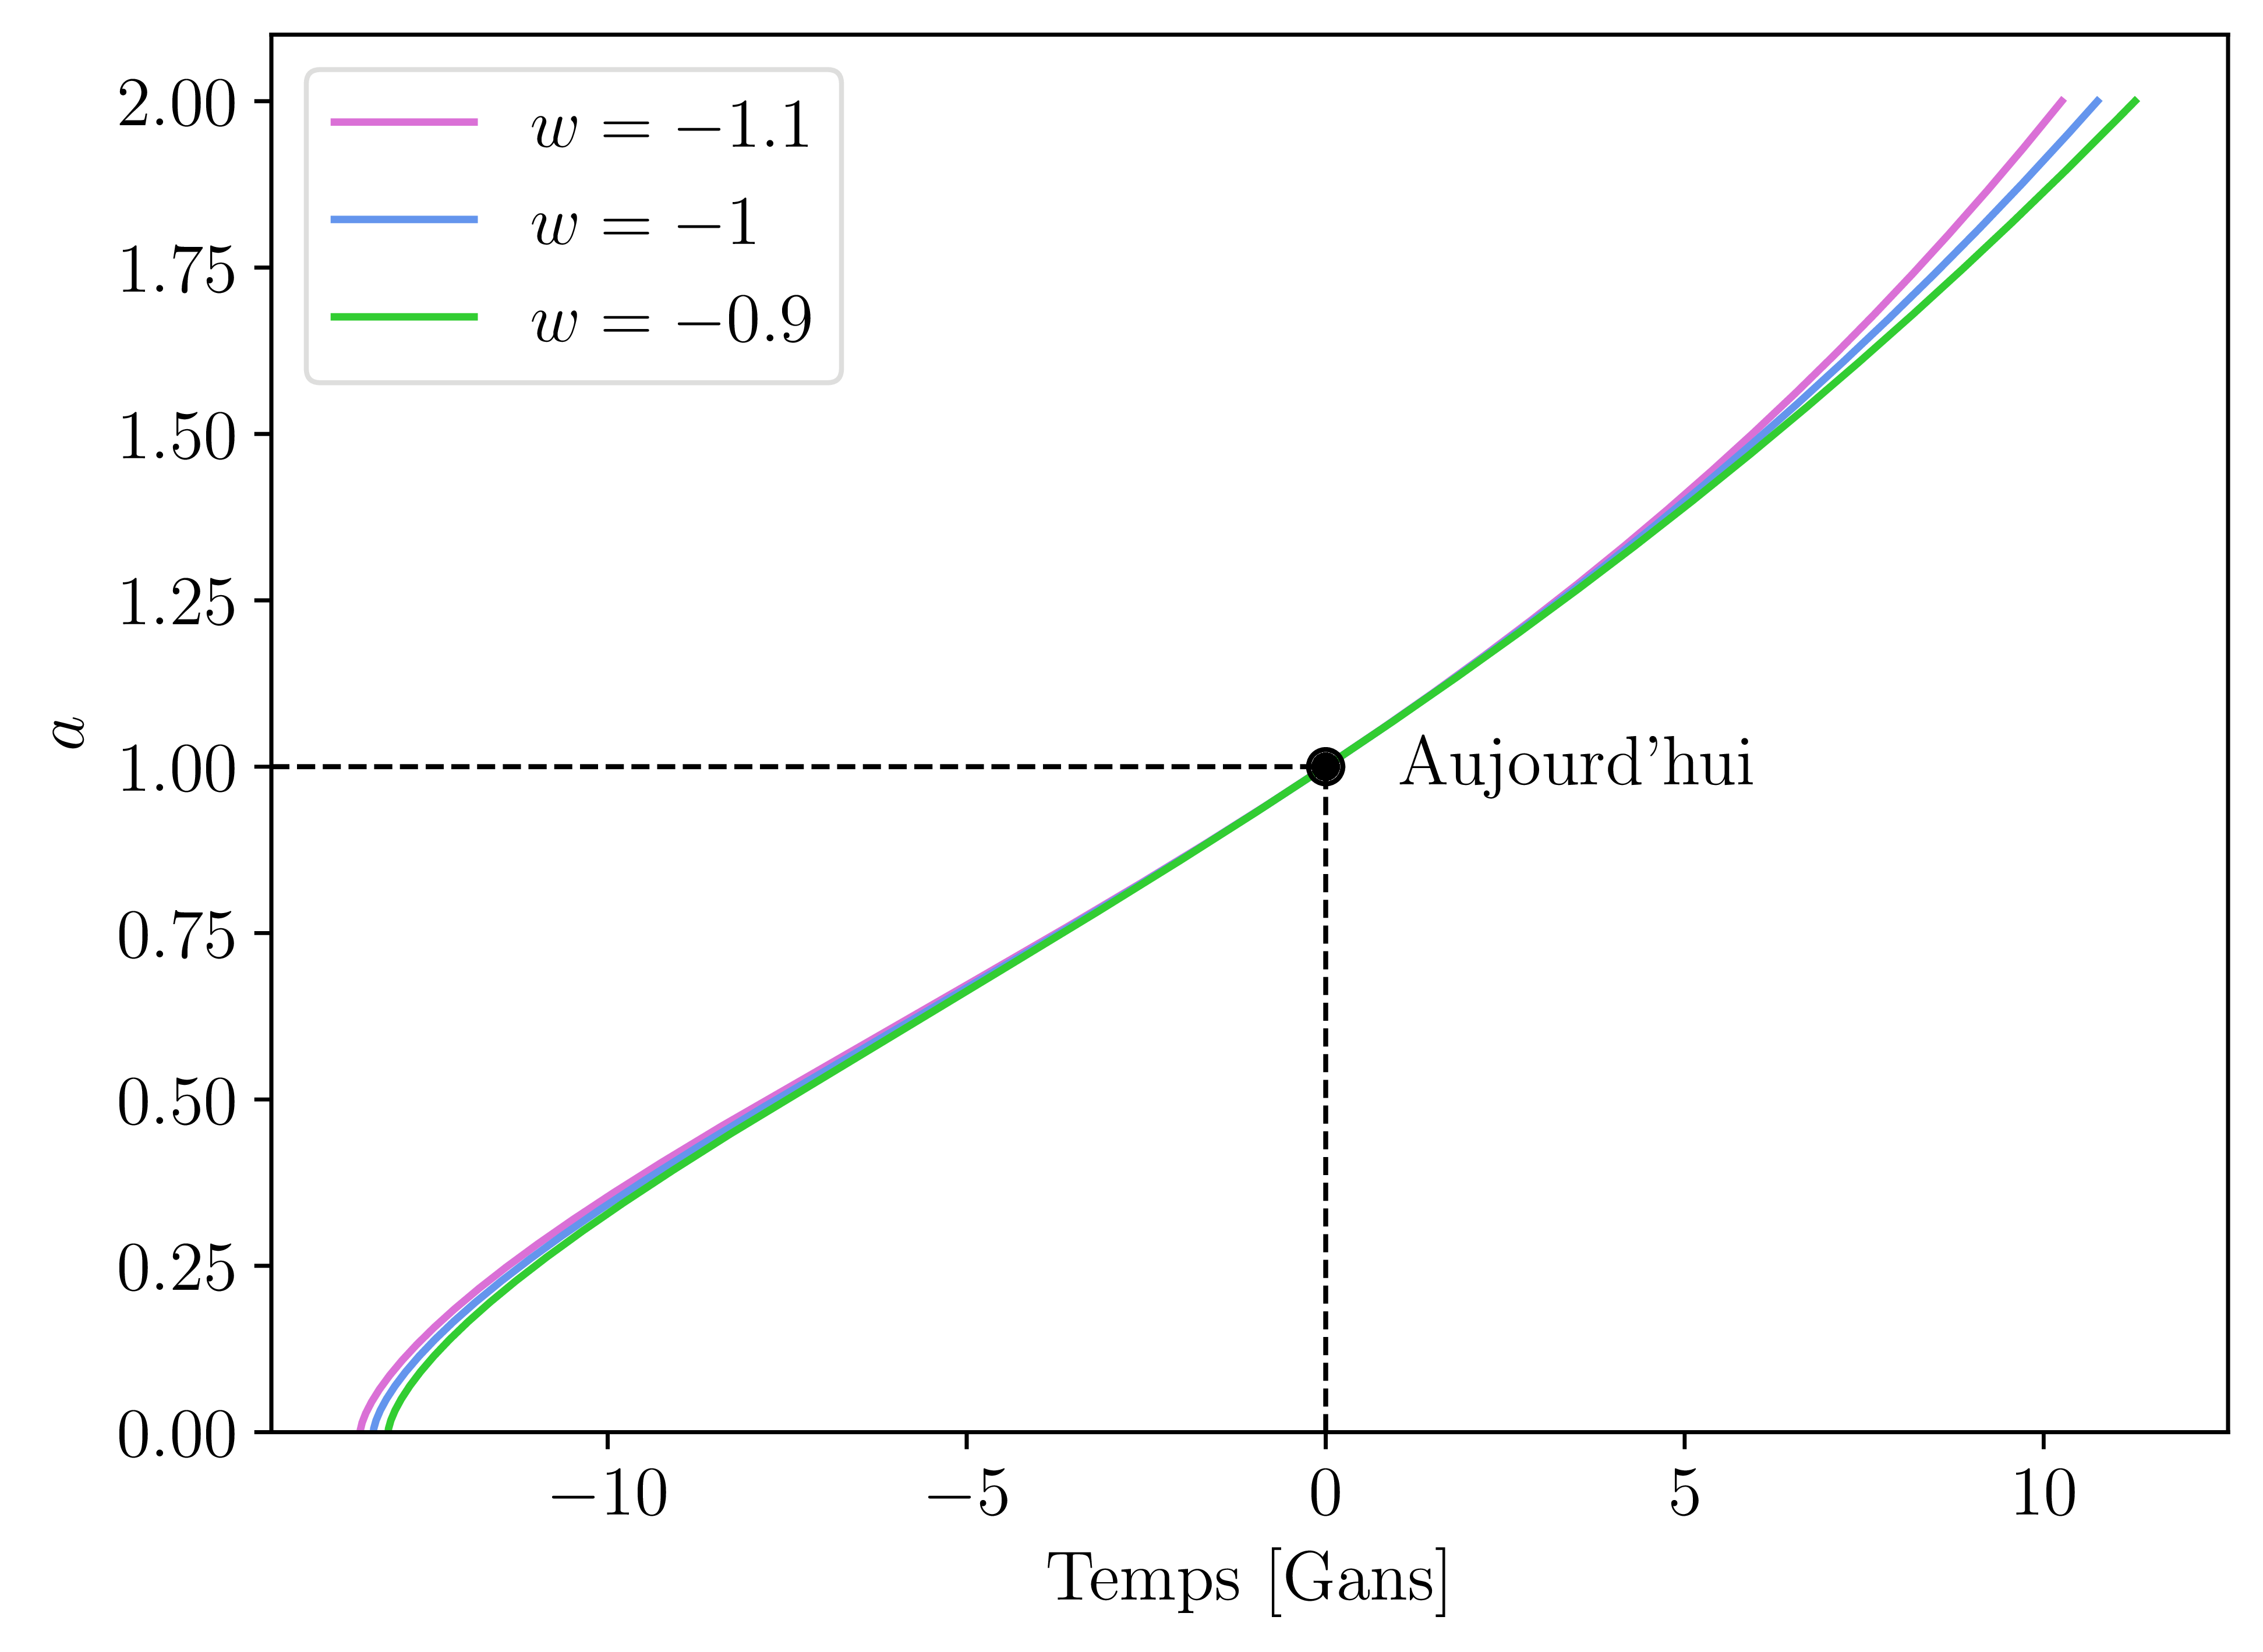
\includegraphics[width=.7\linewidth]{wevol}
    \caption[Effet d'une variation de $w$ sur le facteur d'échelle de
    l'Univers]{Effet d'une variation de $w$ sur le facteur d'échelle de
    l'Univers. Une valeur $< -1$ (par exemple, \num{-1.1}) ferait que l'Univers
est plus âgé que ce que nous croyons, et inversement.}
    \label{fig:wevol}
\end{SCfigure}
\sidecaptionvpos{figure}{t}

Sur la Figure~\ref{fig:wfit}, nous observons que les trois premiers modèles
corrigés de manière cohérente avec leur génération (sur la diagonale donc) sont
tous compatibles avec $w = -1,00$. En revanche, le modèle SK rend incompatible
les autres modèles, que ce soit en l'utilisant pour les données (colonne de
gauche) ou en tant que BiasCor (ligne du haut), introduisant un biais jusqu'à
4\% pour l'échantillon NN\_SK. Si cela ressemble aux résultats de
standardisation, ici cela résulte d'une sous- ou sur-correction systématique
selon l'utilisation de SK, comme nous pouvons le voir Figure~\ref{fig:hr}~: les
modèles donnant $w = \num{-1.00}$ sont équilibrés autour de 0, alors qu'une
sous-correction augmente cette valeur. Les échantillons BP\_NN et NN\_BP, en
revanche, donnent des valeurs compatibles avec \num{-1.00}~; étant donné que les
résultats cosmologiques actuels se basent sur un approche semblable à celle
de~\citetalias{popovic2021a}, ce résultat conforte la validité du modèle NN.

Alors que les trois premiers modèles utilisent la masse comme traceur de la
marche de magnitude et ne contiennent pas d'évolution du vrai $\gamma$ avec le
redshift, le modèle NR utilise l'âge et donc présente une évolution de $\gamma$
avec le redshift. En effet, à $z=0,05$, il est attendu 50\% de jeunes étoiles. À
ce redshift, deux SNe~Ia auront donc soit aucune déviation due à une marche de
magnitude (deux jeunes ou deux vieilles), soit une différence de magnitude entre
elles de \SI{0.130}{mag}, résultant en une moyenne à \SI{0.065}{mag}. À
l'inverse, à haut redshift, les SNe~Ia sont principalement jeunes et la
différence de magnitude entre 2 SNe~Ia tendra donc en moyenne vers \SI{0}{mag}.
Par rapport à la marche de magnitude basée sur la masse, ce modèle sur-évalue la
marche à bas redshift et la sous-évalue à haut redshift. Ceci est visible sur la
Figure~\ref{fig:hr} où, dans la colonne de droite, les points à bas redshift
sont plus bas que dans les autres modèles et les points à haut redshift
($z>0,50$) sont réhaussés. Ceci explique le fait que le modèle NR utilisé comme
données ne fournit pour sa part aucun résultat de $w$ proche de \num{-1.00} dans
la Figure~\ref{fig:wfit}~: \snana\ ne possède pas tous les outils pour prendre
en compte toutes les implications du fait d'utiliser l'âge comme traceur des
propriétés des SNe~Ia. Dans ces conditions, nous observons un biais sur la
mesure de $w$ aux alentours de 5\% si les données présentent effectivement des
corrélations avec l'âge d'une SN mais que la correction utilisée ne le suppose
pas (résultat NR\_BP par exemple), et jusqu'à 8\% si la correction n'inclut
aucune corrélation à la galaxie (résultat NR\_SK).

\subsection{Systématiques dues au choix du modèle de masse}\label{ssec:modsys}

Le choix du modèle de masse diffère principalement dans la fraction retrouvée de
jeunes étoiles en fonction de la masse, dont nous donnons les représentations
graphiques Figure~\ref{fig:fyvM}. Nous exposons ici les différences
cosmologiques dues au choix de la modélisation de la masse, présentées sur les
valeurs de $w$ Figure~\ref{fig:wdiff}.

Nous observons que les différents modèles de masse donnent des fractions de
jeunes étoiles totales similaires entre elles ($\approx 45\%$) mais leurs
distributions ne sont cependant pas les mêmes. En effet, à $M_* >
10^{11}\si{\Msun}$ le modèle SNfsupp est (par construction) dénué de jeunes
étoiles, mais les \wgtmap\ ne favorisent pas ces masses-là donc la différence
n'est pas si notable. En revanche, à $M_* \approx 10^{10}\si{\Msun}$, partie
privilégiée par les \wgtmap, le modèle SEDSNf a la plus haute fraction de jeunes
étoiles (point pentagonal orange, Figure~\ref{fig:fyvM}).

Cette variation pourrait influencer les valeurs de $\alpha$ et $\beta$, mais
ceci n'est pas présent de manière notable. En revanche, elle semble se refléter
dans les valeurs de $w$ comme l'indique la Figure~\ref{fig:wdiff}, où nous
observons une augmentation moyenne des valeurs dans les deux colonnes de
droite. Les observations précédentes restent cependant valables~: le modèle NN
est cohérent avec lui-même et avec le modèle BP, les corrélations entre l'âge
d'une SN et ses propriétés ne sont pas traitées optimalement par \snana\ et le
biais potentiel sur la mesure de $w$ se trouverait entre 4 et 8\%. Nous pouvons
estimer que le choix du modèle de masse contribue à $\approx \num{0.01}$ de la
dispersion de $w$, et que les effets de l'âge sur la marche de magnitude et
l'évolution avec le redshift sont les effets dominants.

\newgeometry{margin=0.5cm}
\begin{landscape}
\begin{figure}[p]
    \centerfloat
    \thisfloatpagestyle{empty}
    \vspace{-0.5cm}
    \begin{subfigure}[]{.30\linewidth}
        \centering
        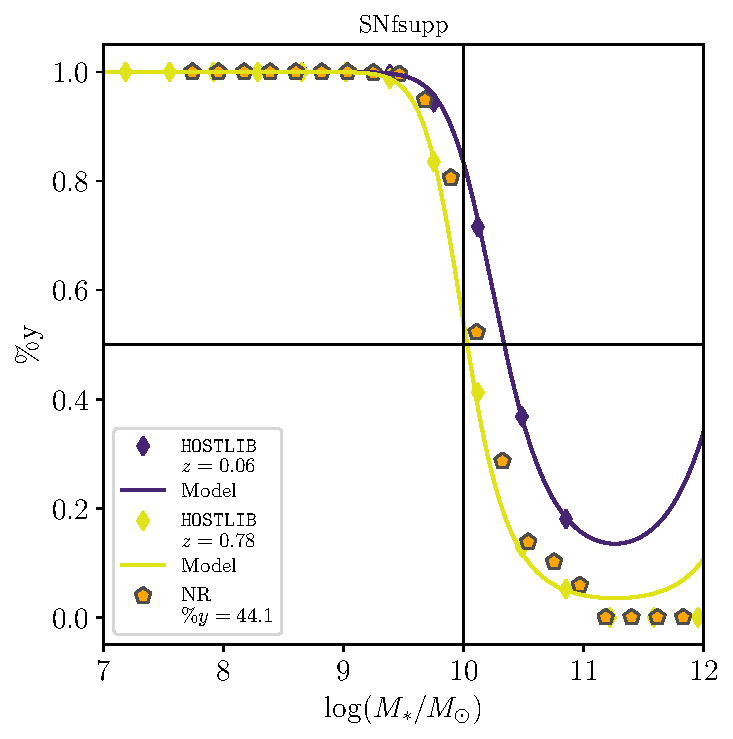
\includegraphics[height=8cm]{snana_diagnostic_fyvM_NRSNFSUPP}
        \caption[Fraction pour SEDSNf]{Fraction pour SNfsupp.}
        \label{fig:fyvMsnfsupp}
    \end{subfigure}
    \centering
    \begin{subfigure}[]{.30\linewidth}
        \centering
        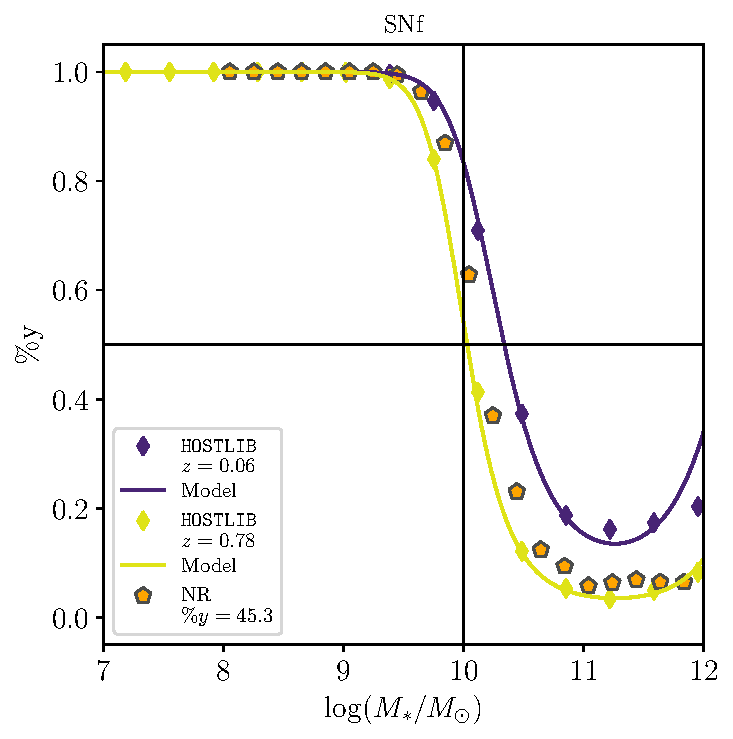
\includegraphics[height=8cm]{snana_diagnostic_fyvM_NRSNF}
        \caption[Fraction pour SEDSNf]{Fraction pour SNf.}
        \label{fig:fyvMsnf}
    \end{subfigure}
    % \hfill
    \begin{subfigure}[]{.30\linewidth}
        \centering
        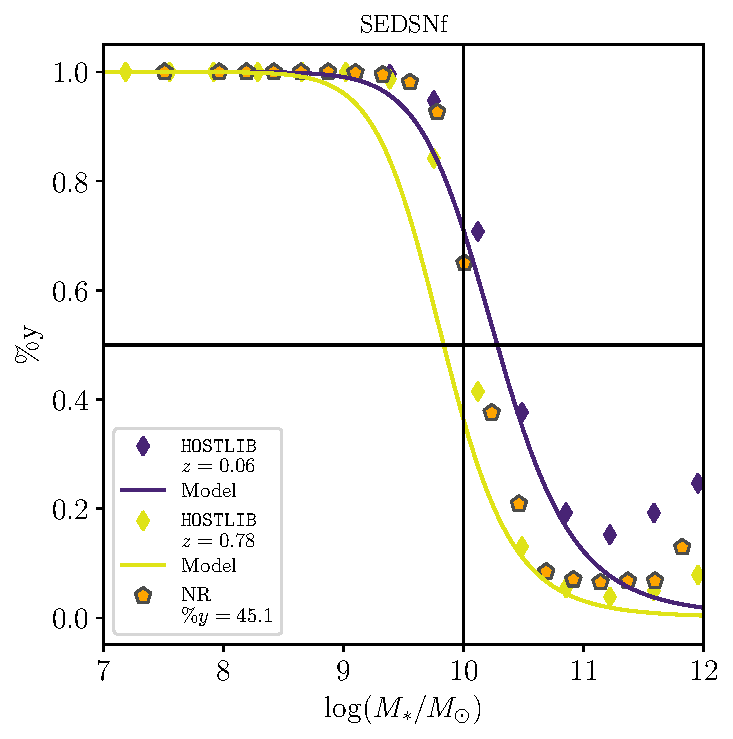
\includegraphics[height=8cm]{snana_diagnostic_fyvM_NRSEDSNF}
        \caption[Fraction pour SEDSNf]{Fraction pour SEDSNf.}
        \label{fig:fyvMsed}
    \end{subfigure}
    \caption[Évolution de la fraction de jeunes étoiles en fonction de la masse
    pour les différents modèles de masse]{\textit{De gauche à droite}~: modèles
        SNfsupp, SNf et SEDSNf. \textit{En violet (jaune)}~: fraction de jeunes
        étoiles en fonction de la masse au redshift moyen de la \hostlib\
        utilisée à hauts (bas) redshifts~; \textit{en orange}~: même fraction
    mais pour l'échantillon simulé NR.}
    \label{fig:fyvM}
\end{figure}

\begin{figure}[h!]
    \centerfloat
    \thisfloatpagestyle{empty}
    % \vspace{-2.2cm}
    \begin{subfigure}[]{.30\linewidth}
        \centering
        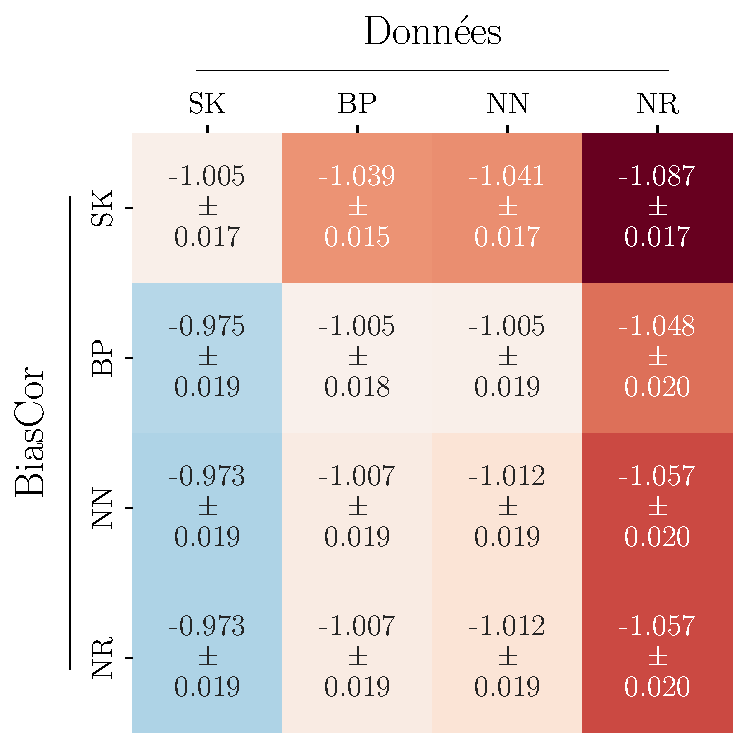
\includegraphics[height=8cm]{wfit_covmat_FULL-SNFSUPP_2}
        \caption[Valeurs de $w$ avec le modèle de masse SNf]{Valeurs de
        $w$ pour SNfsupp.}
        \label{fig:wsnfsupp}
    \end{subfigure}
    % \hfill
    \begin{subfigure}[]{.30\linewidth}
        \centering
        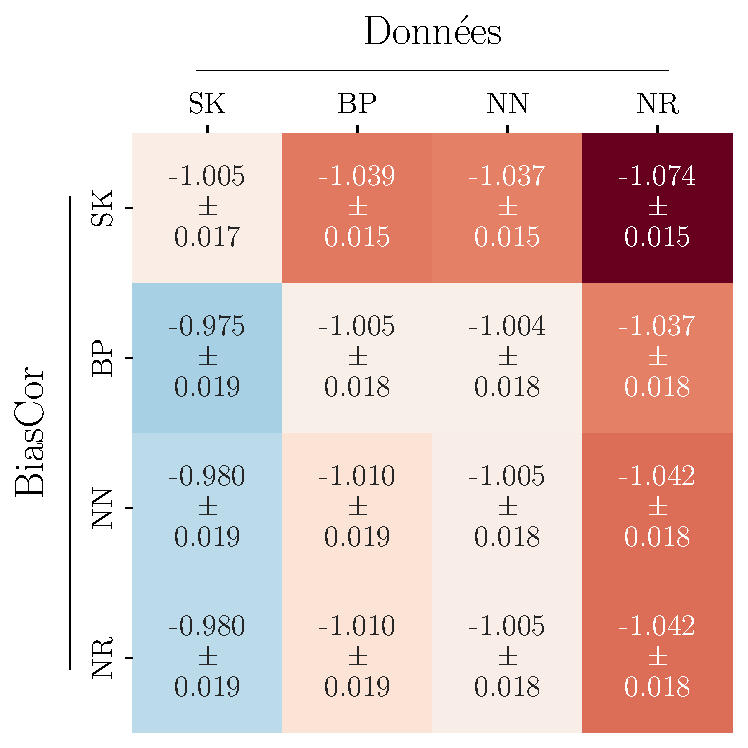
\includegraphics[height=8cm]{wfit_covmat_FULL-SNF_2}
        \caption[Valeurs de $w$ avec le modèle de masse SNf]{Valeurs de
        $w$ pour SNf.}
        \label{fig:wsnf}
    \end{subfigure}
    % \hfill
    \begin{subfigure}[]{.30\linewidth}
        \centering
        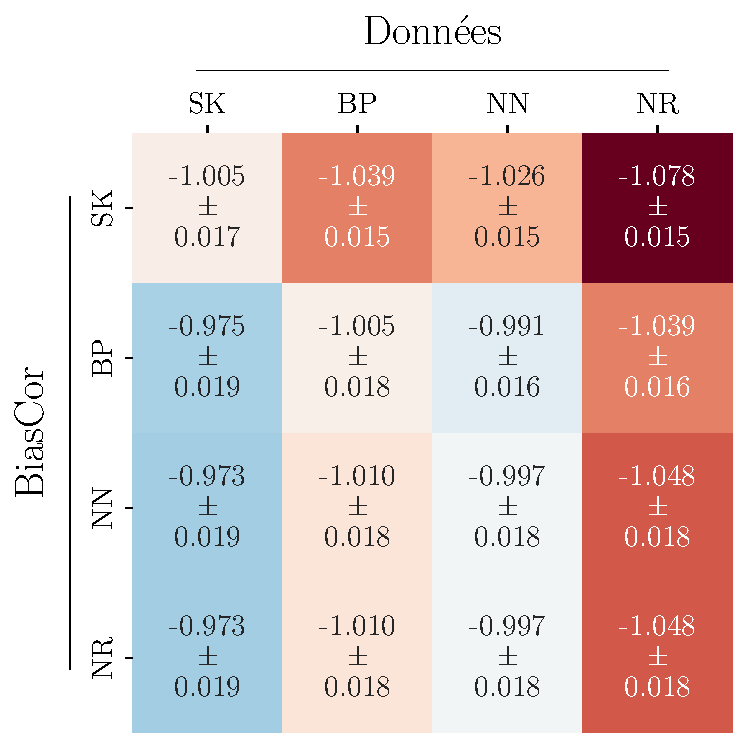
\includegraphics[height=8cm]{wfit_covmat_FULL-SEDSNF_2}
        \caption[Valeurs de $w$ avec le modèle de masse SEDSNf]{Valeurs de
        $w$ pour SEDSNf.}
        \label{fig:wsed}
    \end{subfigure}
    \caption[Résultats cosmologiques~: $w$ selon le modèle de
    masse]{Résultats cosmologiques~: valeurs de $w$ pour les modèles de
        masse SNfsupp \textit{à gauche}, SNf \textit{au milieu} et SEDSNf
    \textit{à droite}.}
    \label{fig:wdiff}
\end{figure}
\end{landscape}
\restoregeometry

\section{Conclusion}\label{sec:simccl}

Nous avons présenté la suite de notre étude de la dérive de la distribution
d'étirement sous-jacente des SNe~Ia en fonction du redshift. Nous avons utilisé
des échantillons de données de masse afin d'établir un modèle de dérive de masse
qui dépend de la fraction attendue des SNe~Ia jeunes et vieilles en fonction du
redshift. Celui-ci nous a permis d'augmenter les \hostlib\
de~\citetalias{popovic2021a} en associant un âge à chacune des entrées, et ce
faisant y changer la corrélation avec l'étirement et la magnitude.

Cette implémentation nous a permis de tester les résultats cosmologiques trouvés
par \snana\ lorsque la correction des données peut être faite de manière
incohérente avec sa génération, en reproduisant les corrélations
de~\citetalias{scolnic2016} et \citetalias{popovic2021a}. Nous obtenons alors 16
échantillons pour lesquels nous avons des valeurs de $\alpha$, $\beta$,
$\gamma_{\rm masse}$ et $w$.

À travers cette analyse et l'implémentation du modèle~\citetalias{nicolas2021}
d'un bout à l'autre du pipeline d'analyse cosmologique \snana, nous
avons pu mettre en lumière les éléments suivants~:
\begin{enumerate}
    \item Nous avons testé la robustesse du modèle d'évolution de l'étirement
        avec le redshift développé dans~\cite{nicolas2021} et présenté au
        Chapitre~\ref{ch:stretch}, qui a été utilisé avec succès pour reproduire
        les sondages totaux et non coupés en redshift~; celui-ci s'est notamment
        avéré être une meilleure description des données à haut redshift que les
        modèles SK ou BP, confortant les indices en faveur de cette évolution~;
    \item chacune des modélisations (SK, BP, NN, NR) sont de bonnes
        représentations des données. La nature ciblée du sondage LOWZ en fait
        un échantillon que nous n'avons pas pu reproduire dans l'état, suivant
        notre approche de modèle prospectif d'étirement, mais il pourrait y être
        ajusté~;
    % \item Nous avons mis en évidence la limite actuelle de l'ensemble de
    %     logiciels \snana\ à prendre en considération l'âge d'une SN comme
    %     traceur de ses propriétés~;
    \item nous avons mis en évidence la limite au fait de considérer la masse
        comme un traceur efficace des propriétés dérivant de l'âge d'une SN~;
    \item nous trouvons que $\gamma_{\rm masse}$ est réduit par rapport à
        $\gamma_{\rm age}$, de manière consistante avec~\cite{briday2022}~;
        % Limitations of taking mass as a tracer of age-derived properties.
        % Gamma_mass is reduced relative to gamma_age, consistant with
        % briday2022.
    \item nous avons montré que les modèles simulés et corrigés de la même
        manière ne présentent pas de biais dans la récupération des valeurs de
        $w$, mais qu'il existe un biais aux alentours de 5\% dans l'hypothèse
        d'une modélisation erronée (NR\_NR)~;
        % If simulate and correct in the same world, no bias; big bias of 5% due
        % to incorrect modeling (NR vs NR)
    \item par rapport à l'état de l'art actuel des analyses cosmologiques
        \citepalias{popovic2021a}, il pourrait y avoir un biais de l'ordre de
        4\% si l'âge constitue le paramètre à l'origine des propriétés des
        SNe~Ia. Cette valeur, compatible avec les incertitudes actuelles, pourra
        se révéler critique à l'ère des futurs grands relevés cosmologiques
        comme LSST qui apporteront rapidement $\approx \num{15000}$ données
        cosmologiques de SNe~Ia.
        % Current cosmo analysis (BP) sees a bias of 4\%, compatible with
        % current error on $w$ but will be critical to LSST/10 000 data…
\end{enumerate}

Ces biais pourraient être corrigés avec l'implémentation de l'âge comme
paramètre décrivant la physique intrinsèque des SNe~Ia, et ouvrirait la voix à
l'étude du biais cosmologique issu de l'utilisation de différents traceurs.

\clearpage

\thispagestyle{plain}
\vspace*{-3cm}
\vfill
\minilof
\vfill
\minilot
\vfill

% \bibliographystyle{../main/aa_url}
% \shorthandoff{:}
% \bibliography{../chapters/99_references}

\end{document}
